\section{Appendix: Proofs}
\subsection{On the Formulation of the Witness Function}
\label{form-witness}
Let $(\mathbf{t}_j)_{j=1}^J$ sampled independently from the $\Gamma$ distribution, then by definition of $d_{p,J}(\cdot,\cdot)$, we have that
\begin{align*}
\label{eq-dlp_J}
    d_{p,J}(P_{XZY},P_{\ddot{X}\otimes Y|Z}):=\left[\frac{1}{J}\sum_{j=1}^J \left|\mu_{P_{XZY},k_{\mathcal{\ddot{X}}}\cdot k_{\mathcal{Y}}}(\mathbf{t}_j)-\mu_{P_{\ddot{X}\otimes Y|Z},k_{\mathcal{\ddot{X}}}\cdot k_{\mathcal{Y}}}(\mathbf{t}_j)\right|^p\right]^{\frac{1}{p}},
\end{align*}
Moreover thanks to Assumption~\ref{assump-kernel}, we have that for any $(\mathbf{t}^{(1)},t^{(2)})\in\mathcal{\ddot{X}}\times\mathcal{Y}$ 
\begin{equation*}
    \mu_{P_{\ddot{X}\otimes Y|Z},k_{\mathcal{\ddot{X}}}\cdot k_{\mathcal{Y}}}(\mathbf{t}^{(1)},t^{(2)})=
    \mathbb{E}_{Z}\left[\mathbb{E}_{\ddot{X}}\left[k_{\mathcal{\ddot{X}}}(\mathbf{t}^{(1)},\ddot{X})|Z\right]
    \mathbb{E}_{Y}\left[k_{\mathcal{Y}}(t^{(2)},Y)|Z\right] \right]\; ,
\end{equation*}
and 
\begin{equation*}
    \mu_{P_{XZY},k_{\mathcal{\ddot{X}}}\cdot k_{\mathcal{Y}}}(\mathbf{t}^{(1)},t^{(2)})=
    \mathbb{E}\left[k_{\mathcal{\ddot{X}}}(\mathbf{t}^{(1)},\ddot{X})
 k_{\mathcal{Y}}(t^{(2)},Y) \right]\; .
\end{equation*}


Let us now introduce the following witness function
\begin{align*}
    \Delta(\mathbf{t}^{(1)},t^{(2)}) :=\mathbb{E}\left[\left(k_{\mathcal{\ddot{X}}}(\mathbf{t}^{(1)},\ddot{X})- \mathbb{E}_{\ddot{X}}\left[k_{\mathcal{\ddot{X}}}(\mathbf{t}^{(1)},\ddot{X})|Z\right]\right)\times\left(k_{\mathcal{Y}}(t^{(2)},Y)- \mathbb{E}_{Y}\left[k_{\mathcal{Y}}(t^{(2)},Y)|Z\right]\right)\right]\;.
\end{align*}
Therefore we obtain that

\begin{align*}
    \Delta(\mathbf{t}^{(1)},t^{(2)}) &=\mathbb{E}\left[k_{\mathcal{\ddot{X}}}(\mathbf{t}^{(1)},\ddot{X})(k_{\mathcal{Y}}(t^{(2)},Y)\right]\\ 
    &- \mathbb{E}\left[k_{\mathcal{\ddot{X}}}(\mathbf{t}^{(1)},\ddot{X})\mathbb{E}_{Y}\left[k_{\mathcal{Y}}(t^{(2)},Y)|Z\right]\right]\\
    &+ \mathbb{E}\left[\mathbb{E}_{\ddot{X}}\left[k_{\mathcal{\ddot{X}}}(\mathbf{t}^{(1)},\ddot{X})|Z\right] \mathbb{E}_{Y}\left[k_{\mathcal{Y}}(t^{(2)},Y)|Z\right] \right]\\
   &- \mathbb{E}\left[\mathbb{E}_{\ddot{X}}\left[k_{\mathcal{\ddot{X}}}(\mathbf{t}^{(1)},\ddot{X})|Z\right]k_{\mathcal{Y}}(t^{(2)},Y)\right]\;.
\end{align*}
Now remarks that
\begin{align*}
    \mathbb{E}\left[k_{\mathcal{\ddot{X}}}(\mathbf{t}^{(1)},\ddot{X})\mathbb{E}_{Y}\left[k_{\mathcal{Y}}(t^{(2)},Y)|Z\right]\right] &= \mathbb{E}\left[\mathbb{E}\left[k_{\mathcal{\ddot{X}}}(\mathbf{t}^{(1)},\ddot{X})\mathbb{E}_{Y}\left[k_{\mathcal{Y}}(t^{(2)},Y)|Z\right]\big|Z\right]\right]\\
    &=\mathbb{E}\left[\mathbb{E}_{Y}\left[k_{\mathcal{Y}}(t^{(2)},Y)|Z\right]  \mathbb{E}_{\ddot{X}}\left[k_{\mathcal{\ddot{X}}}(\mathbf{t}^{(1)},\ddot{X})|Z\right]\right]\;.
\end{align*}
Simiarly, we have that 
\begin{align*}
\mathbb{E}\left[\mathbb{E}_{\ddot{X}}\left[k_{\mathcal{\ddot{X}}}(\mathbf{t}^{(1)},\ddot{X})|Z\right]k_{\mathcal{Y}}(t^{(2)},Y)\right] = \mathbb{E}\left[\mathbb{E}_{Y}\left[k_{\mathcal{Y}}(t^{(2)},Y)|Z\right]  \mathbb{E}_{\ddot{X}}\left[k_{\mathcal{\ddot{X}}}(\mathbf{t}^{(1)},\ddot{X})|Z\right]\right]
\end{align*}
from which follows that 
\begin{align*}
    \Delta(\mathbf{t}^{(1)},t^{(2)}) & = \mathbb{E}\left[k_{\mathcal{\ddot{X}}}(\mathbf{t}^{(1)},\ddot{X})(k_{\mathcal{Y}}(t^{(2)},Y)\right] - \mathbb{E}\left[\mathbb{E}_{Y}\left[k_{\mathcal{Y}}(t^{(2)},Y)|Z\right]  \mathbb{E}_{\ddot{X}}\left[k_{\mathcal{\ddot{X}}}(\mathbf{t}^{(1)},\ddot{X})|Z\right]\right]\\
    &=  \mu_{P_{XZY},k_{\mathcal{\ddot{X}}}\cdot k_{\mathcal{Y}}}(\mathbf{t}^{(1)},t^{(2)}) - \mu_{P_{\ddot{X}\otimes Y|Z},k_{\mathcal{\ddot{X}}}\cdot k_{\mathcal{Y}}}(\mathbf{t}^{(1)},t^{(2)})\;.
\end{align*}


\subsection{Proof of Proposition~\lowercase{\ref{prop:rls-law}}}
\label{prv:rls-law}

\begin{proof} For all $j\in[J]$:
    
\begin{align}
  &\sqrt{n}\widetilde{\Delta}_{n,r}(\mathbf{t}^{(1)}_j,t^{(2)}_j)\\
  &= \sqrt{n}\frac{1}{n}\sum_{i=1}^n  \left(k_{\mathcal{\ddot{X}}}(\mathbf{t}^{(1)}_j,\ddot{x}_i)- h^{(1)}_{j,r}(z_i)\right)\left(k_{\mathcal{Y}}(t^{(2)}_j,y_i)- h^{(2)}_{j,r}(z_i)\right)\nonumber\\
  &= \sqrt{n}\Delta_{n}(\mathbf{t}^{(1)}_j,t^{(2)}_j)\label{eq:term-tcl}\\
  &+\sqrt{n} \frac1n\sum_{i=1}^n\left(k_{\mathcal{\ddot{X}}}(\mathbf{t}^{(1)}_j,\ddot{x}_i)-\mathbb{E}_{\ddot{X}}\left[k_{\mathcal{\ddot{X}}}(\mathbf{t}^{(1)}_j,\ddot{X})|Z=z_i\right]\right)\left(\mathbb{E}_{Y}\left[k_{\mathcal{Y}}(t^{(2)}_j,Y)|Z=z_i\right]- h^{(2)}_{j,r}(z_i)\right)\label{eq:term-cross1}\\
  &+\sqrt{n}\frac1n\sum_{i=1}^n\left(\mathbb{E}_{\ddot{X}}\left[k_{\mathcal{\ddot{X}}}(\mathbf{t}^{(1)}_j,\ddot{X})|Z=z_i\right]-h^{(1)}_{j,r}(z_i)\right)\left(k_{\mathcal{Y}}(t^{(2)}_j,y_i)-\mathbb{E}_{Y}\left[k_{\mathcal{Y}}(t^{(2)}_j,Y)|Z=z_i\right]\right)\label{eq:term-cross2}\\
  &+\sqrt{n}\frac1n\sum_{i=1}^n\left(\mathbb{E}_{\ddot{X}}\left[k_{\mathcal{\ddot{X}}}(\mathbf{t}^{(1)}_j,\ddot{X})|Z=z_i\right]-h^{(1)}_{j,r}(z_i)\right)\left(\mathbb{E}_{Y}\left[k_{\mathcal{Y}}(t^{(2)}_j,Y)|Z=z_i\right]-h^{(2)}_{j,r}(z_i)\right)\label{eq:term-cross3}
\end{align} 

Let us treat the four terms of this decomposition. The term~\eqref{eq:term-tcl} has been treated by Propostion~\ref{prop:oracle-law}, and satisfies, under the null hypothesis $H_0$
\begin{align*}
\sqrt{n}\Delta_{n}&(\mathbf{t}_j^{(1)},t_j^{(2)})\\
&\to_{n\to\infty} \mathcal{N}\left(0,\mathbb{E}\left[\left(k_{\mathcal{\ddot{X}}}(\mathbf{t}^{(1)}_j,\ddot{X})-\mathbb{E}_{\ddot{X}}\left[k_{\mathcal{\ddot{X}}}(\mathbf{t}^{(1)}_j,\ddot{X})|Z\right]\right)\left(k_{\mathcal{Y}}(t^{(2)}_j,Y)-\mathbb{E}_{Y}\left[k_{\mathcal{Y}}(t^{(2)}_j,Y)|Z\right]\right)\right]\right)
\end{align*}

Let us now show that the last term~\eqref{eq:term-cross3} converges towards $0$ in probability. Let us denote for all $j$, $e^{(1)}_{j}:z\to\mathbb{E}_{\ddot{X}}\left[k_{\mathcal{\ddot{X}}}(\mathbf{t}^{(1)}_j,\ddot{X})|Z=z\right] $ and $e^{(2)}_{j}:z\to\mathbb{E}_{Y}\left[k_{\mathcal{\ddot{X}}}(t^{(2)}_j,Y)|Z=z\right]$, both elements of $ H_{\mathcal{Z}}$ by Assumption~\ref{ass:source}. Then we have, for all $i\in[n]$:

\begin{align*}
   \left(e^{(1)}_{j}(z_i)-h^{(1)}_{j,r}(z_i)\right)\left(e^{(2)}_{j}(z_i)-h^{(2)}_{j,r}(z_i)\right)=\langle\left(e^{(1)}_{j}-h^{(1)}_{j,r}\right)\otimes\left(e^{(2)}_{j}-h^{(2)}_{j,r}\right), k_{\mathcal{Z}}(z_i,\cdot)\otimes k_{\mathcal{Z}}(z_i,\cdot)\rangle.
\end{align*}
Then we deduce, by denoting: $\mu_{ZZ} := \mathbb{E}\left[ k_{\mathcal{Z}}(Z,\cdot)k_{\mathcal{Z}}(Z,\cdot)\right]$ and $\hat{\mu}_{ZZ}:=\frac1n\sum_{i=1}^n k_{\mathcal{Z}}(z_i,\cdot)k_{\mathcal{Z}}(z_i,\cdot)$, that
\begin{align*}
    \frac1n\sum_{i=1}^n\left(\mathbb{E}_{\ddot{X}}\left[k_{\mathcal{\ddot{X}}}(\mathbf{t}^{(1)}_j,\ddot{X})|Z=z_i\right]-h^{(1)}_{j,r}(z_i)\right)\left(\mathbb{E}_{Y}\left[k_{\mathcal{Y}}(t^{(2)}_j,Y)|Z=z_i\right]-h^{(2)}_{j,r}(z_i)\right)\\
    = \langle\left(e^{(1)}_{j}-h^{(1)}_{j,r}\right)\otimes\left(e^{(2)}_{j}-h^{(2)}_{j,r}\right),\frac{1}{n}\sum_{i=1}^n k_{\mathcal{Z}}(z_i,\cdot)\otimes k_{\mathcal{Z}}(z_i,\cdot)\rangle\\
    =\langle\left(e^{(1)}_{j}-h^{(1)}_{j,r}\right)\otimes\left(e^{(2)}_{j}-h^{(2)}_{j,r}\right),\mu_{ZZ}\rangle+\langle\left(e^{(1)}_{j}-h^{(1)}_{j,r}\right)\otimes\left(e^{(2)}_{j}-h^{(2)}_{j,r}\right),\hat{\mu}_{ZZ}-\mu_{ZZ}\rangle\;.
\end{align*}
Then remarks that:
\begin{align*}
    \lvert\langle\left(e^{(1)}_{j}-h^{(1)}_{j,r}\right)\otimes\left(e^{(2)}_{j}-h^{(2)}_{j,r}\right),\mu_{ZZ}\rangle\rvert&=\lvert\mathbb{E}_Z\left[\left(e^{(1)}_{j}(Z)-h^{(1)}_{j,r}(Z)\right)\left(e^{(2)}_{j}(Z)-h^{(2)}_{j,r}(Z)\right)\right]\rvert\\
    &\leq \lVert e^{(1)}_{j}-h^{(1)}_{j,r}\rVert_{L^2(P_Z)} \lVert  e^{(2)}_{j}-h^{(2)}_{j,r}\rVert_{L^2(P_Z)} 
\end{align*}
Under the Assumptions~\ref{ass:spectrum}-\ref{ass:source}, for $\lambda_{r} = \frac{1}{r^{\beta+\gamma}}$, we have, using the results from~\cite{fischer2020sobolev}: $\lVert  e^{(1)}_{j}-h^{(1)}_{j,r}\rVert_{L^2(P_Z)}^2\leq \frac{C\tau^2}{r^{\frac{\beta}{\beta+\gamma}}}$ with probability $1-4e^{-\tau}$ and  $ \lVert e^{(2)}_{j}-h^{(2)}_{j,r}\rVert_{L^2(P_Z)}^2 \leq \frac{C\tau^2}{r^{\frac{\beta}{\beta+\gamma}}}$ with probability $1-4e^{-\tau}$, for some constant $C$ independent from $n$ and $\tau$. then by union bound, we deduce with probability $1-8e^{-\tau}$ we have:
\begin{align*}
    \sqrt{n}\lvert\langle\left(e^{(1)}_{j}-h^{(1)}_{j,r}\right)\otimes\left(e^{(2)}_{j}-h^{(2)}_{j,r}\right),\mu_{ZZ}\rangle\rvert\leq \sqrt{n}\frac{C^2\tau^4}{r^{\frac{\beta}{\beta+\gamma}}}
\end{align*}

Then, if $\sqrt{n}\in o(r^{\frac{\beta}{\beta+\gamma}})$, we have:
$ \sqrt{n}\lvert\langle\left(e^{(1)}_{j}-h^{(1)}_{j,r}\right)\otimes\left(e^{(2)}_{j}-h^{(2)}_{j,r}\right),\mu_{ZZ}\rangle\rvert\to 0$ in probability when $n\to\infty$. Moreover:
\begin{align*}
    \lvert \left(e^{(1)}_{j}-h^{(1)}_{j,r}\right)\otimes\left(e^{(2)}_{j}-h^{(2)}_{j,r}\right),\hat{\mu}_{ZZ}-\mu_{ZZ}\rangle\rvert\leq \lVert e^{(1)}_{j}-h^{(1)}_{j,r}\rVert_{ H_\mathcal{Z}} \lVert e^{(2)}_{j}-h^{(2)}_{j,r}\rVert_{ H_\mathcal{Z}}\lVert\hat{\mu}_{ZZ}-\mu_{ZZ}\rVert_{ H_\mathcal{Z}\otimes H_\mathcal{Z}}\; ,
\end{align*}
and by Markov inequality, $\lVert\hat{\mu}_{ZZ}-\mu_{ZZ}\rVert_{H_\mathcal{Z}\otimes H_\mathcal{Z}} \leq \sqrt{\frac{C'}{n\delta}}$ with probability $1-\delta$ for some constant $C'$. Moreover, under Assumption~\ref{ass:spectrum}-\ref{ass:source}, we have $\lVert e^{(1)}_{j}-h^{(1)}_{j,r}\rVert_{ H_\mathcal{Z}}\to 0$ and $\lVert e^{(2)}_{j}-h^{(2)}_{j,r}\rVert_{ H_\mathcal{Z}}\to 0$ in probability. Then, we deduce that $\sqrt{n}\lvert \langle\left(e^{(1)}_{j}-h^{(1)}_{j,r}\right)\otimes\left(e^{(2)}_{j}-h^{(2)}_{j,r}\right),\hat{\mu}_{ZZ}-\mu_{ZZ}\rangle\rvert\to 0$ in probability. Finally, the term~\eqref{eq:term-cross3} goes to $0$ in probability. 



The terms~\eqref{eq:term-cross1} and~\eqref{eq:term-cross2} are similar and can be treated the same way. We only focus on the term~\eqref{eq:term-cross1}. For all $i\in[n]$:
\begin{align*}
\lvert\frac1n\sum_{i=1}^n\left(k_{\mathcal{\ddot{X}}}(\mathbf{t}^{(1)}_j,\ddot{x}_i)-\mathbb{E}_{\ddot{X}}\left[k_{\mathcal{\ddot{X}}}(\mathbf{t}^{(1)}_j,\ddot{X})|Z=z_i\right]\right)\left(\mathbb{E}_{Y}\left[k_{\mathcal{Y}}(t^{(2)}_j,Y)|Z=z_i\right]- h^{(2)}_{j,r}(z_i)\right)\rvert\\
  =\lvert\frac1n\sum_{i=1}^n\langle k_{\mathcal{\ddot{X}}}(t^{(1)}_j,\cdot),k_{\mathcal{\ddot{X}}}(\ddot{x}_i,\cdot)-\mathbb{E}_{\ddot{X}}\left[k_{\mathcal{\ddot{X}}}(\ddot{X},\cdot)|Z=z_i\right]\rangle_{ H_\mathcal{\ddot{X}}}
  \langle e^{(2)}_{j}-h^{(2)}_{j,r},k_{\mathcal{Z}}(z_i,\cdot)\rangle_{ H_\mathcal{Z}}\rvert\\
  =\lvert\frac1n\sum_{i=1}^n\langle k_{\mathcal{\ddot{X}}}(t^{(1)},\cdot)\otimes \left(e^{(2)}_{j}-h^{(2)}_{j,r}\right),\left(k_{\mathcal{\ddot{X}}}(\ddot{x}_i,\cdot)-\mathbb{E}_{\ddot{X}}\left[k_{\mathcal{\ddot{X}}}(\ddot{X},\cdot)|Z=z_i\right]\right)\otimes k_{\mathcal{Z}}(z_i,\cdot)\rangle_{ H_\mathcal{\ddot{X}}\otimes H_\mathcal{Z}}\rvert\\
  =\lvert\langle k_{\mathcal{\ddot{X}}}(t^{(1)},\cdot)\otimes \left(e^{(2)}_{j}-h^{(2)}_{j,r}\right),\frac1n\sum_{i=1}^n\left(k_{\mathcal{\ddot{X}}}(\ddot{x}_i,\cdot)-\mathbb{E}_{\ddot{X}}\left[k_{\mathcal{\ddot{X}}}(\ddot{X},\cdot)|Z=z_i\right]\right)\otimes k_{\mathcal{Z}}(z_i,\cdot)\rangle_{ H_\mathcal{\ddot{X}}\otimes H_\mathcal{Z}}\rvert\\
  \leq \lVert k_{\mathcal{\ddot{X}}}(t^{(1)},\cdot)\rVert_{ H_\mathcal{\ddot{X}}}\lVert e^{(2)}_{j}-h^{(2)}_{j,r}\rVert_{H_\mathcal{Z}}\left(\lVert \hat{\mu}^1_{\ddot{X}Z}-\mu_{\ddot{X}Z}\rVert_{ H_\mathcal{\ddot{X}}\otimes H_\mathcal{Z}}+ \lVert\hat{\mu}^2_{\ddot{X}}-\mu_{\ddot{X}Z}\rVert_{ H_\mathcal{\ddot{X}}\otimes H_\mathcal{Z}}\right)
\end{align*}
where: $\hat{\mu}^1_{\ddot{X}Z} := \frac1n\sum_{i=1}^nk_{\mathcal{\ddot{X}}}(\ddot{x}_i,\cdot)\otimes k_{\mathcal{Z}}(z_i,\cdot)$, $\hat{\mu}^2_{\ddot{X}Z}:=\frac1n\sum_{i=1}^n\mathbb{E}_{\ddot{X}}\left[k_{\mathcal{\ddot{X}}}(\ddot{X},\cdot)|Z=z_i\right]\otimes k_{\mathcal{Z}}(z_i,\cdot)$, and $\mu_{\ddot{X}Z}:=\mathbb{E}\left[k_{\mathcal{Y}}(y,\cdot)k_{\mathcal{Z}}(z,\cdot)\right]$.

By the law of large numbers, we have: $\hat{\mu}^1_{\ddot{X}Z}$ and $\hat{\mu}^2_{\ddot{X}Z}$ converge almost surely towards $\mu_{\ddot{X}Z}$. Moreover by Markov inequality, $\lVert\hat{\mu}^1_{\ddot{X}Z}-\mu_{\ddot{X}Z}\rVert_{ H_\mathcal{\ddot{X}}\otimes H_\mathcal{Z}} \leq \sqrt{\frac{C}{n\delta}}$ with probability $1-\delta$, and  $\lVert\hat{\mu}^2_{\ddot{X}Z}-\mu_{\ddot{X}Z}\rVert_{ H_\mathcal{\ddot{X}}\otimes H_\mathcal{Z}} \leq \sqrt{\frac{C}{n\delta}}$ with probability $1-\delta$. Then with probability $1-2\delta$, $\sqrt{n}\left(\lVert\hat{\mu}^1_{\ddot{X}Z}-\mu_{\ddot{X}Z}\rVert_{ H_\mathcal{\ddot{X}}\otimes H_\mathcal{Z}}+\lVert\hat{\mu}^2_{\ddot{X}Z}-\mu_{\ddot{X}Z}\rVert_{ H_\mathcal{\ddot{X}}\otimes H_\mathcal{Z}} \right)\leq2\sqrt{\frac{C}{\delta}}$. Moreover, under Assumption~\ref{ass:spectrum}-\ref{ass:source}, using the results from~\cite{fischer2020sobolev}, we have that $\lVert e^{(2)}_{j}-h^{(2)}_{j,r}\rVert_{H_\mathcal{Z}}$ converges towards $0$ in probability. Then the term~\eqref{eq:term-cross1}
converges in probability towards $0$. The same reasoning holds for~\eqref{eq:term-cross2}. 

Finally, by Slutsky's Lemma:
\begin{align*}
    \sqrt{n}\widetilde{\Delta}_{n,r}&(\mathbf{t}^{(1)}_j,t^{(2)}_j)\\
    &\to_{n\to\infty} \mathcal{N}\left(0,\mathbb{E}\left[\left(k_{\mathcal{\ddot{X}}}(\mathbf{t}^{(1)}_j,\ddot{X})-\mathbb{E}_{\ddot{X}}\left[k_{\mathcal{\ddot{X}}}(\mathbf{t}^{(1)}_j,\ddot{X})|Z\right]\right)\left(k_{\mathcal{Y}}(t^{(2)}_j,Y)-\mathbb{E}_{Y}\left[k_{\mathcal{Y}}(t^{(2)}_j,Y)|Z\right]\right)\right]\right).
\end{align*}
Now we have:
\begin{align*}
    \widetilde{\mathbf{S}}_{n,r}=\left(\widetilde{\Delta}_{n,r}(\mathbf{t}^{(1)}_j,t^{(2)}_j)\right)_{j\in[J]}=\left(\Delta_{n}(\mathbf{t}^{(1)}_j,t^{(2)}_j)\right)_{j\in[J]}+ \left(\widetilde{\Delta}_{n,r}(\mathbf{t}^{(1)}_j,t^{(2)}_j)-\Delta_{n}(\mathbf{t}^{(1)}_j,t^{(2)}_j)\right)_{j\in[J]}
\end{align*}
 and  we have shown that $\sqrt{n}\left(\widetilde{\Delta}_{n,r_n}(\mathbf{t}^{(1)}_j,t^{(2)}_j)-\Delta_{n}(\mathbf{t}^{(1)}_j,t^{(2)}_j)\right)_{j\in[J]}$ goes to $0$ in probability. Then by Slutsky Lemma and Proposition~\ref{prop:oracle-law}, we get: $\widetilde{\mathbf{S}}_{n,r_n}\to\mathcal{N}\left(0,\bm{\Sigma}\right)$.%, under $H_0$ we have:
% \begin{align*}
%     \left(\mu_{\text{w},r}(\mathbf{t}^{(1)}_j,t^{(2)}_j)\right)_{j\in[J]}\to \mathcal{N}\left(0,\Sigma_J\right).
% \end{align*}
%with $\Sigma_J=\left(\mathbb{E}\left[\left(k_{\mathcal{\ddot{X}}}(\mathbf{t}_i^{(1)},\ddot{X})-\mathbb{E}_{\ddot{X}}\left[k_{\mathcal{\ddot{X}}}(\mathbf{t}_i^{(1)},\ddot{X})|Z\right]\right)\left(k_{\mathcal{Y}}(t_j^{(2)},Y)-\mathbb{E}_{Y}\left[k_{\mathcal{Y}}(t_j^{(2)},Y)|Z\right]\right)\right]\right)_{i,j\in[J]}$. Then by Slutsky Lemma, we get: $\hat{V}_n\to\mathcal{N}\left(0,\Sigma_J\right)$.

Let $r>0$. Under $H_1$, $\mathbf{\mathbf{S}}_{n,r_n}\to \mathbf{S}\neq 0$. Let consider a realization of $(\mathbf{t}^{(1)}_j,t_j^{(2)})_{j\in[J]}$ such that $\lVert \mathbf{S}\rVert_p\neq 0$. So $P(n^{p/2}\lVert \mathbf{S}_{n,r_n}\rVert_p\geq r)\to 1$ as $n\to\infty$ because $\lVert \mathbf{S}\rVert_p\neq 0$.
\end{proof}
\newpage
\subsection{Proof of Proposition~\lowercase{\ref{prop:norm-law}}}
\label{prv:norm-law}
\begin{proof}
First notice that:
\begin{align*}
  \bm{\widetilde{\Sigma}}_{n,r}&:=\frac{1}{n}\sum_{i=1}^n \widetilde{\mathbf{u}}_{i,r}\widetilde{\mathbf{u}}_{i,r}^T+\delta_n \text{Id}_J  \\
  &=  \bm{\widehat{\Sigma}}_{n}+\frac1n\sum_{i=1}^n \widehat{\mathbf{u}}_{i}\left(\widetilde{\mathbf{u}}_{i,r}-\widehat{\mathbf{u}}_{r}\right)^T+\frac1n\sum_{i=1}^n \left(\widetilde{\mathbf{u}}_{i,r}-\widehat{\mathbf{u}}_{r}\right)\widehat{\mathbf{u}}_{i}^T\\
  &+\frac1n\sum_{i=1}^n\left(\widetilde{\mathbf{u}}_{i,r}-\widehat{\mathbf{u}}_{r}\right) \left(\widetilde{\mathbf{u}}_{i,r}-\widehat{\mathbf{u}}_{r}\right)^T+\delta_n \text{Id}_J
\end{align*}

By the law of large numbers, we get that under $H_0$: $\bm{\widehat{\Sigma}}_{n}\to\bm{\Sigma}$. Moreover:
\begin{align*}
    \left[\frac1n\sum_{i=1}^n \widehat{\mathbf{u}}_{i}\left(\widetilde{\mathbf{u}}_{i,r}-\widehat{\mathbf{u}}_{r}\right)^T\right]_{kl} = \frac{1}{n}\sum_{i=1}^n\left(k_{\mathcal{Y}}(t_k^{(2)},y_i)-\mathbb{E}_{Y}\left[k_{\mathcal{Y}}(t_k^{(2)},Y)|Z=z_i\right]\right)\left(\mathbb{E}_{\ddot{X}}\left[k_{\mathcal{\ddot{X}}}(\mathbf{t}_l^{(1)},\ddot{X})|Z=z_i\right]-h^{(1)}_{l,r}(z_i)\right)
\end{align*}
which has been proven to converge in probability to $0$ in the proof of Proposition~\ref{prop:rls-law}. Then $\frac1n\sum_{i=1}^n \widehat{\mathbf{u}}_{i}\left(\widetilde{\mathbf{u}}_{i,r}-\widehat{\mathbf{u}}_{r}\right)^T$ converges in probability to $0$. Similarly $\frac1n\sum_{i=1}^n \left(\widetilde{\mathbf{u}}_{i,r}-\widehat{\mathbf{u}}_{r}\right)\widehat{\mathbf{u}}_{i}^T$ and  $\frac1n\sum_{i=1}^n\left(\widetilde{\mathbf{u}}_{i,r}-\widehat{\mathbf{u}}_{r}\right) \left(\widetilde{\mathbf{u}}_{i,r}-\widehat{\mathbf{u}}_{r}\right)^T$ also converge in probability to $0$. Then by Slutsky Lemma, $ \bm{\widetilde{\Sigma}}_{n,r}$ converges in probability to $\bm{\Sigma}$. By Slutsky's lemma (again) and by Propostion~\ref{prop:rls-law}, we have that:
$\bm{\widetilde{\Sigma}}_{n,r}^{-1}\bm{\widetilde{S}}_{n,r}$ converges to a standard gaussian distribution $\mathcal{N}(0,\text{Id})$. The second part of the proposition is the same than the proof of Proposition~\ref{prop:rls-law}.
\end{proof}
% Let denote the operator $R:\ddot{\mathcal{X}}\rightarrow\mathcal{Z}$ defined as:
% $R =\left(\Sigma^{k_\mathcal{Z},k_\mathcal{Z}}_{p_{ZZ}}\right)^{-1}\Sigma^{k_\mathcal{Z},k_{\ddot{\mathcal{X}}}}_{p_{Z\ddot{X}}}$. 
% Let denote $R_M$ defined using the approximated random features kernel spaces: $R_M =\left(\Sigma^{k_{\mathcal{Z},M},k_{\mathcal{Z},M}}_{p_{ZZ}}\right)^{-1}\Sigma^{k_{\mathcal{Z},M},k_{\ddot{\mathcal{X}},M}}_{p_{Z\ddot{X}}}$
% Let show that: for all $u,v$
% \begin{align*}
%     \langle R_M k_{\ddot{\mathcal{X}},M}(u,\cdot),k_{\mathcal{Z},M}(v,\cdot)\rangle_{ H_{\mathcal{Z},M}}\to_{M\to\infty}     \langle R k_{\ddot{\mathcal{X}}}(u,\cdot),k_{\mathcal{Z}}(v,\cdot)\rangle_{ H_\mathcal{Z}}\text{ in probability} 
% \end{align*}

% We have:
% \begin{align*}
%     \langle R k_{\ddot{\mathcal{X}}}(u,\cdot),k_{\mathcal{Z}}(v,\cdot)\rangle_{ H_{\mathcal{Z}}} =     \langle \left(\Sigma^{k_\mathcal{Z},k_\mathcal{Z}}_{p_{ZZ}}\right)^{-1/2}R k_{\ddot{\mathcal{X}}}(u,\cdot),\left(\Sigma^{k_\mathcal{Z},k_\mathcal{Z}}_{p_{ZZ}}\right)^{-1/2}k_{\mathcal{Z}}(v,\cdot)\rangle_{L^2(p_Z)}
% \end{align*}

% \begin{align*}
%     \langle R_M k_{\ddot{\mathcal{X}},M}(u,\cdot),k_{\mathcal{Z},M}(v,\cdot)\rangle_{ H_{\mathcal{Z},M}} =     \langle \left(\Sigma^{k_{\mathcal{Z},M},k_{\mathcal{Z},M}}_{p_{ZZ}}\right)^{-1/2}R_M k_{\ddot{\mathcal{X}},M}(u,\cdot),\left(\Sigma^{k_{\mathcal{Z},M},k_{\mathcal{Z},M}}_{p_{ZZ}}\right)^{-1/2}k_{\mathcal{Z},M}(v,\cdot)\rangle_{L^2(p_Z)} 
% \end{align*}

% One can notice that

% \begin{align*}
%     \Sigma^{k_{\mathcal{Z},M},k_{\mathcal{Z},M}}_{p_{ZZ}} = \frac1M \sum_{i=1}^M \xi_i
% \end{align*}
% where $\xi_i = \phi_{\theta_i}\otimes\phi_{\theta_i}$ are i.i.d. copies. And $\Sigma^{k_{\mathcal{Z},M},k_{\mathcal{Z},M}}_{p_{ZZ}} = \mathbb{E}(\xi_1)$. Then:
% \begin{align*}
%     \mathbb{P}\left[\lVert\Sigma^{k_{\mathcal{Z},M},k_{\mathcal{Z},M}}_{p_{ZZ}}- \Sigma^{k_{\mathcal{Z}},k_{\mathcal{Z}}}_{p_{ZZ}}\rVert_{HS(L^2(p_Z),L^2(p_Z))} \geq \epsilon\right]&\leq  \frac{\mathbb{E}\left[\lVert\Sigma^{k_{\mathcal{Z},M},k_{\mathcal{Z},M}}_{p_{ZZ}}- \Sigma^{k_{\mathcal{Z}},k_{\mathcal{Z}}}_{p_{ZZ}}\rVert_{HS(L^2(p_Z),L^2(p_Z))}^2 \right]}{\epsilon^2}\\
%     &\leq \frac{1}{M\epsilon}\mathbb{E}\left[\lVert \xi_1-\mathbb{E}(x_1)\rVert_{HS(L^2(p_Z),L^2(p_Z))}\right]
% \end{align*}
% Then we deduce:
% \begin{align*}
% \lVert\Sigma^{k_{\mathcal{Z},M},k_{\mathcal{Z},M}}_{p_{ZZ}}- \Sigma^{k_{\mathcal{Z}},k_{\mathcal{Z}}}_{p_{ZZ}}\rVert_{HS(L^2(p_Z),L^2(p_Z))} \to 0 \text{ in probability.}
% \end{align*}

% \begin{align*}
% \lVert\Sigma^{k_{\mathcal{Z},M},k_{\ddot{\mathcal{X}},M}}_{p_{Z\ddot{X}}}- \Sigma^{k_{\mathcal{Z}},k_{\ddot{\mathcal{X}}}}_{p_{Z\ddot{X}}}\rVert_{HS(L^2(p_{\ddot{X}}),L^2(p_Z))} \to 0 \text{ in probability.}
% \end{align*}

% Then one can show that:

% \begin{align*}
% \lVert\left(\Sigma^{k_{\mathcal{Z},M},k_{\mathcal{Z},M}}_{p_{ZZ}}\right)^{-1/2}- \left(\Sigma^{k_{\mathcal{Z}},k_{\mathcal{Z}}}_{p_{ZZ}}\right)^{-1/2} \rVert_{HS(L^2(p_Z),L^2(p_Z))}\to 0 \text{ in probability.}
% \end{align*}

% \begin{align*}
% \lVert \left(\Sigma^{k_{\mathcal{Z},M},k_{\mathcal{Z},M}}_{p_{ZZ}}\right)^{-1/2}R_M- \left(\Sigma^{k_{\mathcal{Z}},k_{\mathcal{Z}}}_{p_{ZZ}}\right)^{-1/2} R\rVert_{HS(L^2(p_{\ddot{X}}),L^2(p_Z))} \to 0 \text{ in probability.}
% \end{align*}
% Moreover since $k_{\ddot{\mathcal{X}},M}$ converges uniformly in probability towards $k_{\ddot{\mathcal{X}}}$ on the compact $\ddot{\mathcal{X}}$. The same argument holds for $k_{\mathcal{Z},M}$. Then:
% \begin{align*}
%     \lVert k_{\ddot{\mathcal{X}},M}(v,\cdot)-k_{\ddot{\mathcal{X}}}(v,\cdot)\rVert_{L^2(p_{\ddot{\mathcal{X}}})}\to 0\text{ in probability}
% \end{align*}
% \begin{align*}
%     \lVert k_{\mathcal{Z}}(u,\cdot)-k_{\mathcal{Z}}(u,\cdot)\rVert_{L^2(p_{\mathcal{Z}})}\to 0\text{ in probability}
% \end{align*}
% Then:

% \begin{align*}
%   \lvert \langle R_M k_{\ddot{\mathcal{X}},M}(u,\cdot),k_{\mathcal{Z},M}(v,\cdot)\rangle_{ H_{\mathcal{Z},M}}-    \langle R k_{\ddot{\mathcal{X}}}(u,\cdot),k_{\ddot{\mathcal{X}}}(v,\cdot)\rangle_{ H_\mathcal{Z}}\rvert\\
%   \leq \lVert \left(\Sigma^{k_{\mathcal{Z},M},k_{\mathcal{Z},M}}_{p_{ZZ}}\right)^{-1/2}R_M- \left(\Sigma^{k_{\mathcal{Z}},k_{\mathcal{Z}}}_{p_{ZZ}}\right)^{-1/2} R\rVert_{HS(L^2(p_{\ddot{X}}),L^2(p_Z))} \lVert k_{\ddot{\mathcal{X}},M}(u,\cdot)\rVert_{L^2(p_{\ddot{X}})} \lVert k_{\mathcal{Z},M}(v,\cdot)\rVert_{L^2(p_{Z})} \lVert\left(\Sigma^{k_{\mathcal{Z},M},k_{\mathcal{Z},M}}_{p_{ZZ}}\right)^{-1/2}\rVert_{HS(L^2(p_{Z}),L^2(p_Z))} \\
%   +\lVert\left(\Sigma^{k_{\mathcal{Z},M},k_{\mathcal{Z},M}}_{p_{ZZ}}\right)^{-1/2}- \left(\Sigma^{k_{\mathcal{Z}},k_{\mathcal{Z}}}_{p_{ZZ}}\right)^{-1/2} \rVert_{HS(L^2(p_{Z}),L^2(p_Z))}\lVert k_{\ddot{\mathcal{X}},M}(u,\cdot)\rVert_{L^2(p_{\ddot{X}})} \lVert k_{\mathcal{Z},M}(v,\cdot)\rVert_{L^2(p_{Z})} \lVert\left(\Sigma^{k_{\mathcal{Z}},k_{\mathcal{Z}}}_{p_{ZZ}}\right)^{-1/2} R\rVert_{HS(L^2(p_{\ddot{X}}),L^2(p_Z))} \\
%   +\lVert k_{\ddot{\mathcal{X}},M}(u,\cdot)- k_{\ddot{\mathcal{X}}}(u,\cdot)\rVert_{L^2(p_{\ddot{X}})}\lVert\left(\Sigma^{k_{\mathcal{Z}},k_{\mathcal{Z}}}_{p_{ZZ}}\right)^{-1/2} \rVert_{HS(L^2(p_{Z}),L^2(p_Z))}\lVert k_{\mathcal{Z},M}(v,\cdot)\rVert_{L^2(p_Z)} \lVert\left(\Sigma^{k_{\mathcal{Z}},k_{\mathcal{Z}}}_{p_{ZZ}}\right)^{-1/2} R\rVert_{HS(L^2(p_{\ddot{X}}),L^2(p_Z))}\\
%   +\lVert k_{\mathcal{Z},M}(v,\cdot)- k_{\mathcal{Z}}(v,\cdot)\rVert_{L^2(p_{Z})}\lVert\left(\Sigma^{k_{\mathcal{Z}},k_{\mathcal{Z}}}_{p_{ZZ}}\right)^{-1/2} \rVert_{HS(L^2(p_{Z}),L^2(p_Z))} \lVert k_{\ddot{\mathcal{X}}}(u,\cdot)\rVert_{L^2(p_{\ddot{X}})} \lVert\left(\Sigma^{k_{\mathcal{Z}},k_{\mathcal{Z}}}_{p_{ZZ}}\right)^{-1/2} R\rVert_{HS(L^2(p_{\ddot{X}}),L^2(p_Z))}
% \end{align*}

% Finally we have shown that for all $u,v$:
% \begin{align*}
%     \langle R_M k_{\ddot{\mathcal{X}},M}(u,\cdot),k_{\mathcal{Z},M}(v,\cdot)\rangle_{ H_{\mathcal{Z},M}}\to_{M\to\infty}     \langle R k_{\ddot{\mathcal{X}}}(u,\cdot),k_{\mathcal{Z}}(v,\cdot)\rangle_{ H_\mathcal{Z}}\text{ in probability} 
% \end{align*}

% \section{A note on finding }
% \label{sec-theoritical-findings}

\section{Appendix: Additional Experiments}
\subsection{A note on the computation of Oracle statistic in Figure~\ref{fig-illustation-theory}}
\label{sec-theoritical-findings}

To compute the oracle statistic we needed to compute exactly the conditional expectation implied in our statistic. In the case of gaussian kernels and gaussian distributed data for $Z$, the computation of this conditional expectation is reduced to the computation of moment-generating function of a non-centered $\chi^2$ distribution.

\newpage
\subsection{Choice of the rank regression $r$}
\label{sec-rank-rn}
In this experiment, we show the effect of the rank regression $r$ on the performances of our proposed method. For that purpose, in Figure~\ref{fig-rn-dependence}, we consider the two problems presented in~\eqref{exp-strobl-h0} and~\eqref{exp-strobl-h1}  with Gaussian noises and show the type-I and type-II when varying the ratio $r/n$ for multiple sample size $n$. We observe that the rank $r$ does not affect the power of the method, however we observe that the type-I error decreases as the ratio increases. Therefore the rank $r$ allows in practice to deal with the tradeoff between the computational time and the control of the type-I error.

\begin{figure*}[ht]
\begin{tabular}{cccc} 
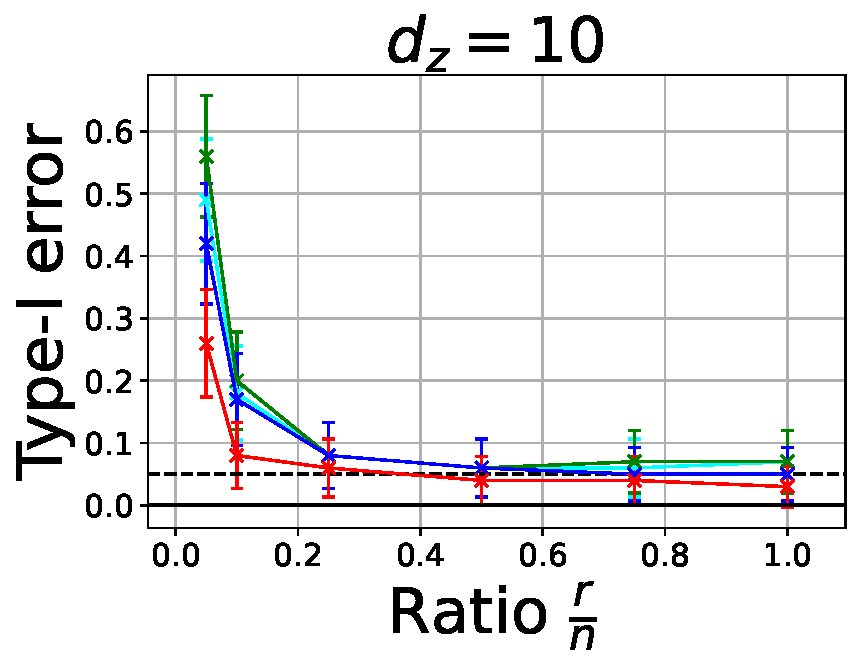
\includegraphics[height=3cm]{sections/appendix/independence_testing_kernel/figures_r_n/fig_ours_r_n_typeI.pdf}& 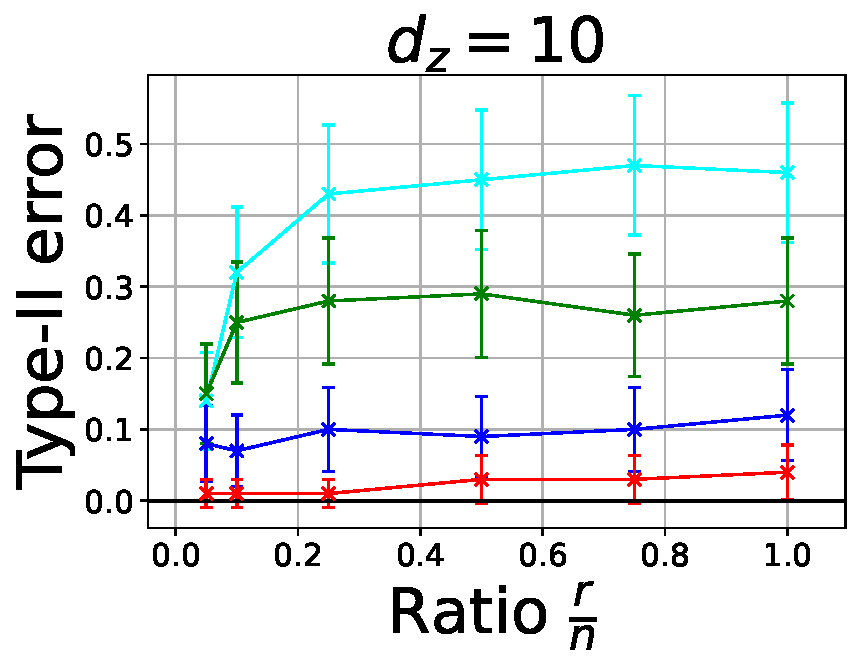
\includegraphics[height=3cm]{sections/appendix/independence_testing_kernel/figures_r_n/fig_ours_r_n_typeII.pdf}&
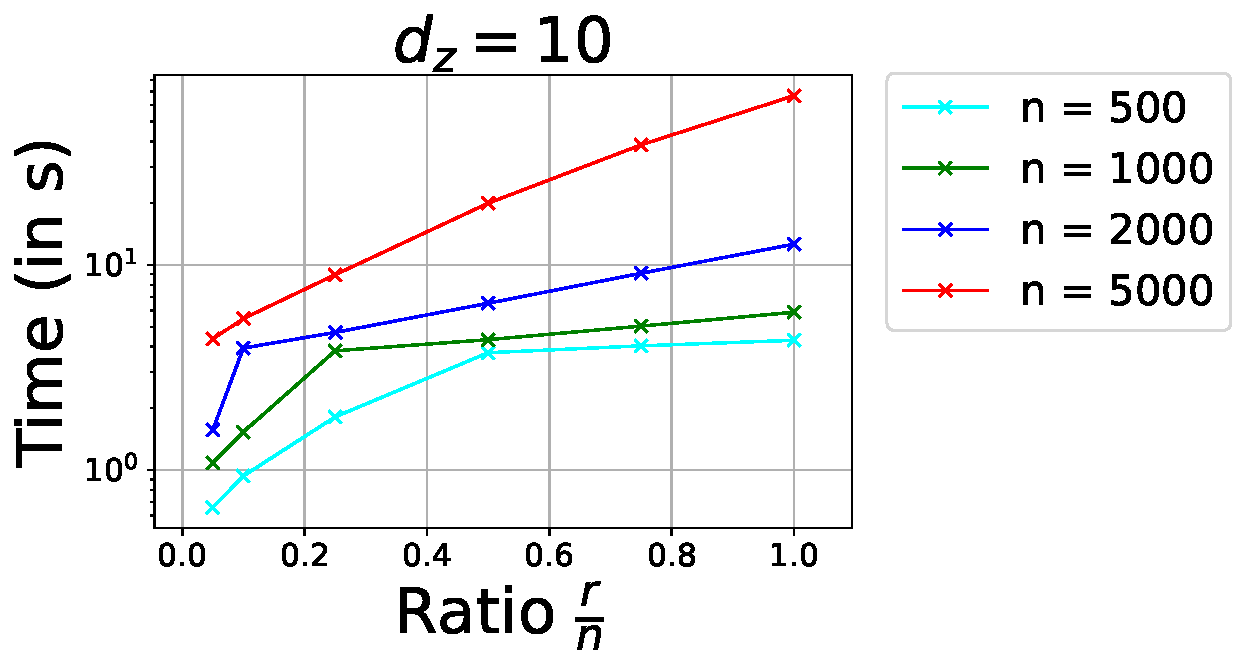
\includegraphics[height=3cm]{sections/appendix/independence_testing_kernel/figures_r_n/fig_ours_r_n_time.pdf}\\
\end{tabular}
\caption{Comparison of the type-I error at level $\alpha=0.05$ (dashed line) and the type-II error (lower is better) of our test procedure with other SoTA tests on the two problems presented in~\eqref{exp-strobl-h0} and~\eqref{exp-strobl-h1}  with Gaussian noises. Each point in the figures is obtained by repeating the experiment for 100 independent trials. (\emph{Left, Middle}): type-I and type-II errors obtained by each test when varying the ratio regression rank/total number of samples for different number of samples. (\emph{Right}): time in seconds (log-scale) to compute the statistic  when varying the ratio regression rank/total number of samples for different number of samples.
\label{fig-rn-dependence}}
\vspace{-0.5cm}
\end{figure*}





\newpage
\subsection{Additional experiments on Problems~\eqref{exp-strobl-h0} and~\eqref{exp-strobl-h1}}
\label{sec-exp-storbl}
\vspace{-0.2cm}
\subsubsection{Gaussian Case}
\vspace{-0.4cm}
% In this section, we provide an additional comparison of the KS statistic and the AUPC obtained by the different tests when the data is generated from the models defined in Eq.~\eqref{exp-strobl-h0} and Eq.~\eqref{exp-strobl-h1}, respectively, focusing on a high dimensional setting. Figure~\ref{fig-exp-li-ks-dim} demonstrates that, in most cases, our method indeed outperforms the existing tests both in terms of the KS and AUPC performance metrics.

\begin{figure*}[h]
\begin{tabular}{cccc} 
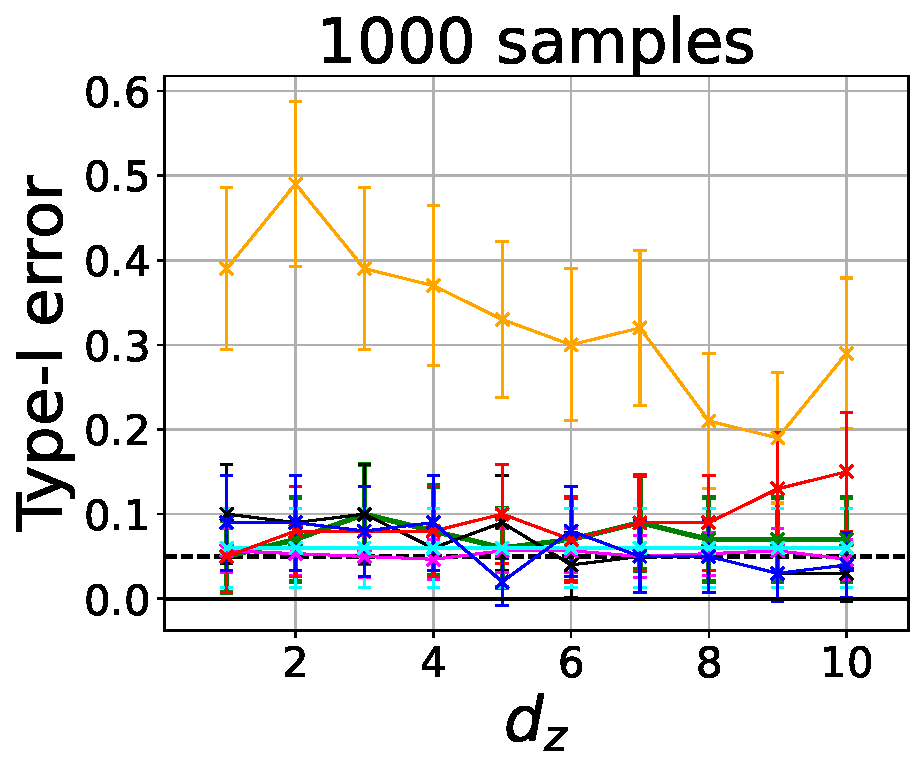
\includegraphics[height=2.2cm]{sections/appendix/independence_testing_kernel/figures_strobl_gaussian/nsamples_fixed_1000_strobl_dim_1_10_typeI.pdf}& 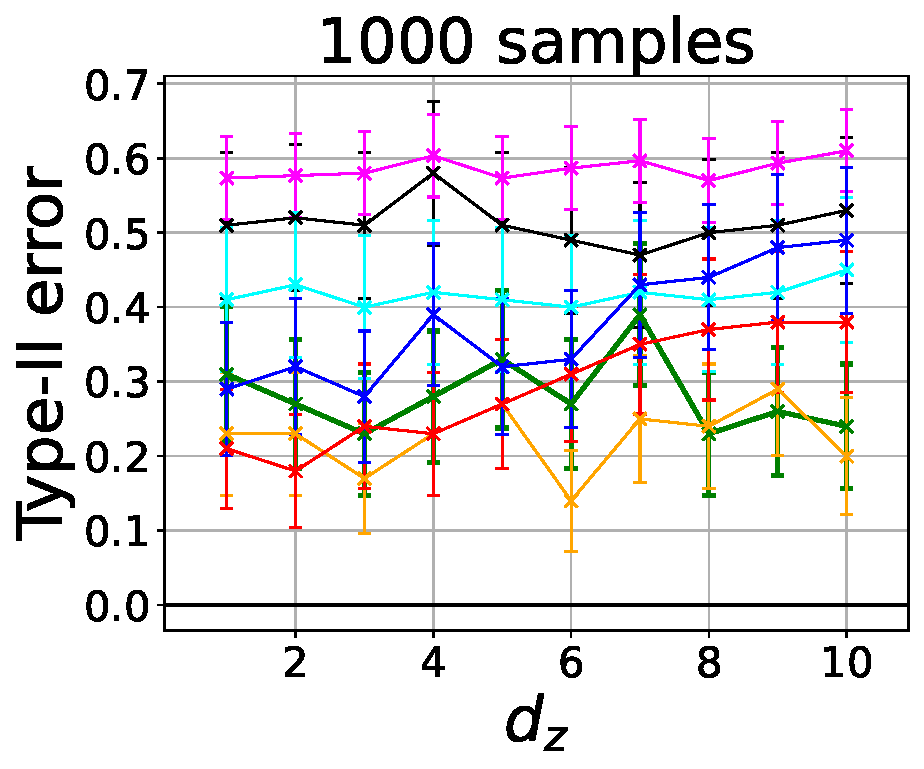
\includegraphics[height=2.2cm]{sections/appendix/independence_testing_kernel/figures_strobl_gaussian/nsamples_fixed_1000_strobl_dim_1_10_typeII.pdf} & 
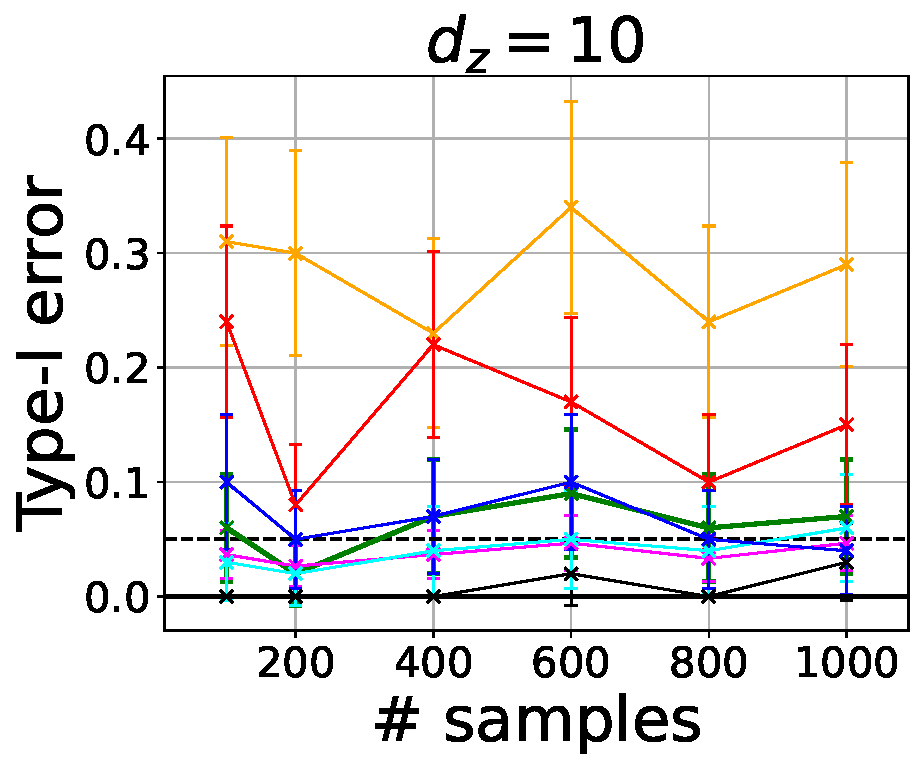
\includegraphics[height=2.2cm]{sections/appendix/independence_testing_kernel/figures_strobl_gaussian/dim_fixed_10_strobl_typeI.pdf}& 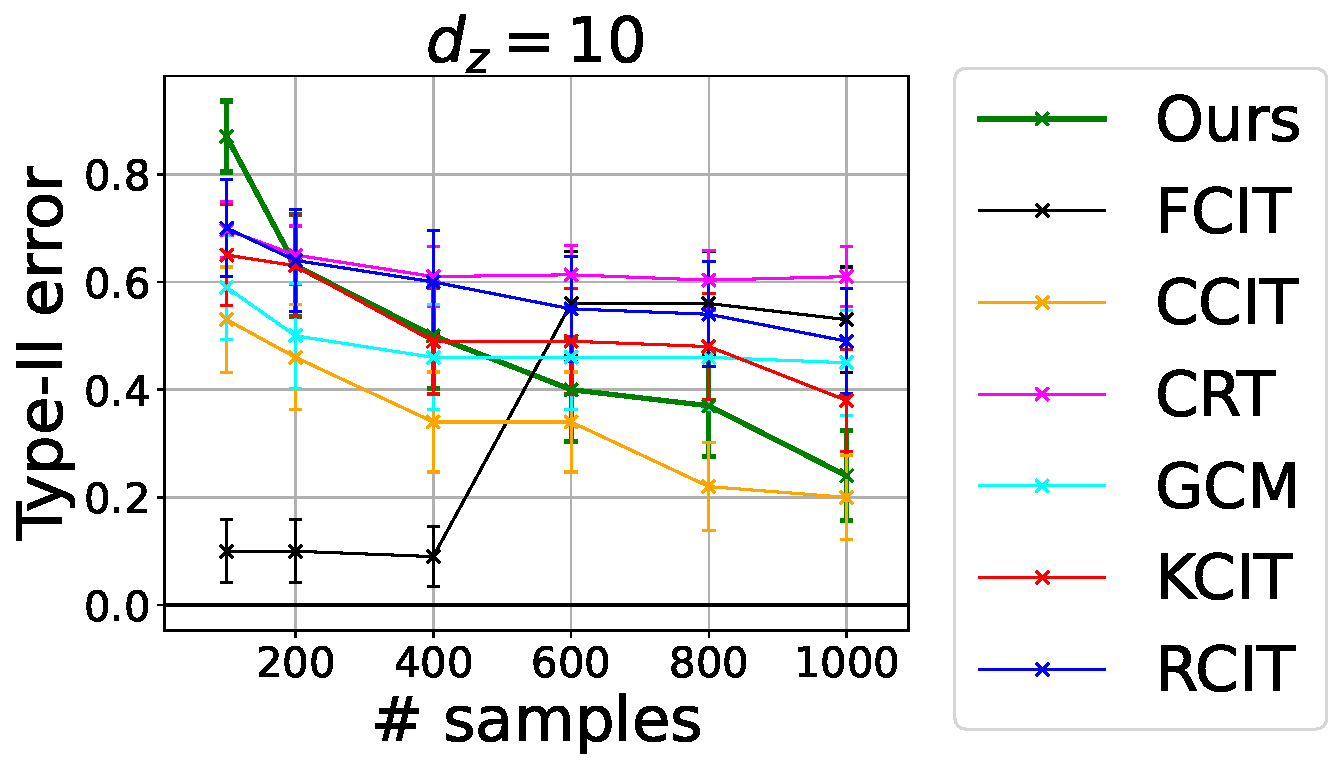
\includegraphics[height=2.2cm]{sections/appendix/independence_testing_kernel/figures_strobl_gaussian/dim_fixed_10_strobl_typeII.pdf}
\end{tabular}
\caption{Comparison of the type-I error at level $\alpha=0.05$ (dashed line) and the type-II error (lower is better) of our test procedure with other SoTA tests on the two problems presented in~\eqref{exp-strobl-h0} and~\eqref{exp-strobl-h1}  with Gaussian noises. Each point in the figures is obtained by repeating the experiment for 100 independent trials. (\emph{Left, middle-left}): type-I and type-II errors obtained by each test when varying the dimension $d_z$ from 1 to 10; here, the number of samples $n$ is fixed and equals to $1000$. (\emph{Middle-right, right}): type-I and type-II errors obtained by each test when varying the number of samples $n$ from 100 to 1000; the dimension $d_z$ is fixed and equals $10$. 
\label{fig-exp-strobl-type-supp}}
\vspace{-0.5cm}
\end{figure*}




\begin{figure*}[ht]
\begin{tabular}{cccc} 
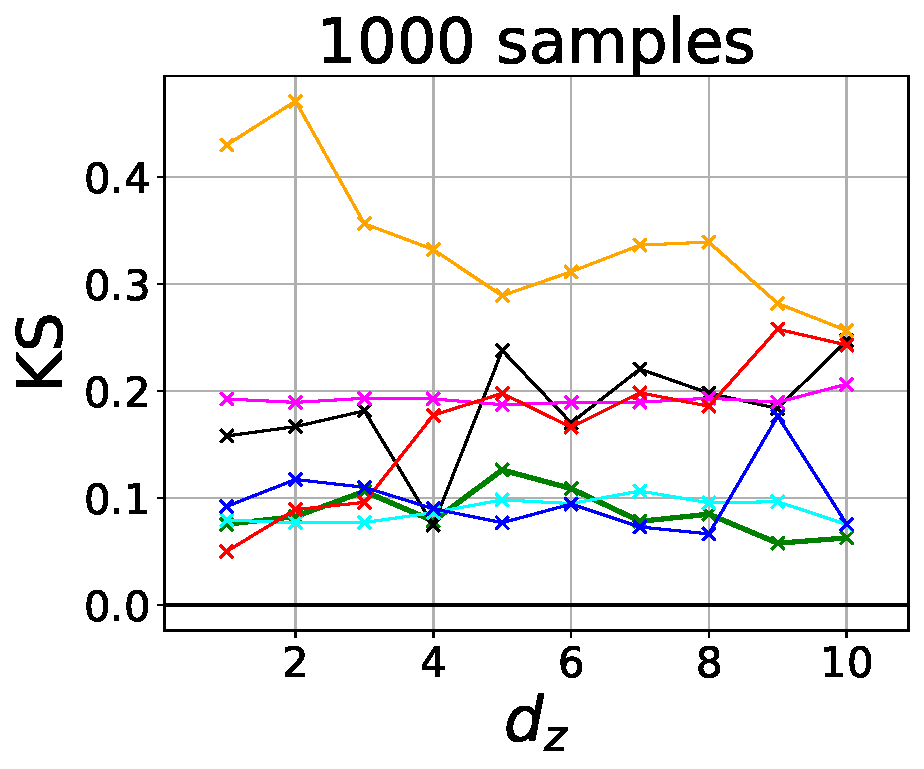
\includegraphics[height=2.2cm]{sections/appendix/independence_testing_kernel/new_figures/nsamples_fixed_1000_strobl_dim_1_10_ks.pdf}& 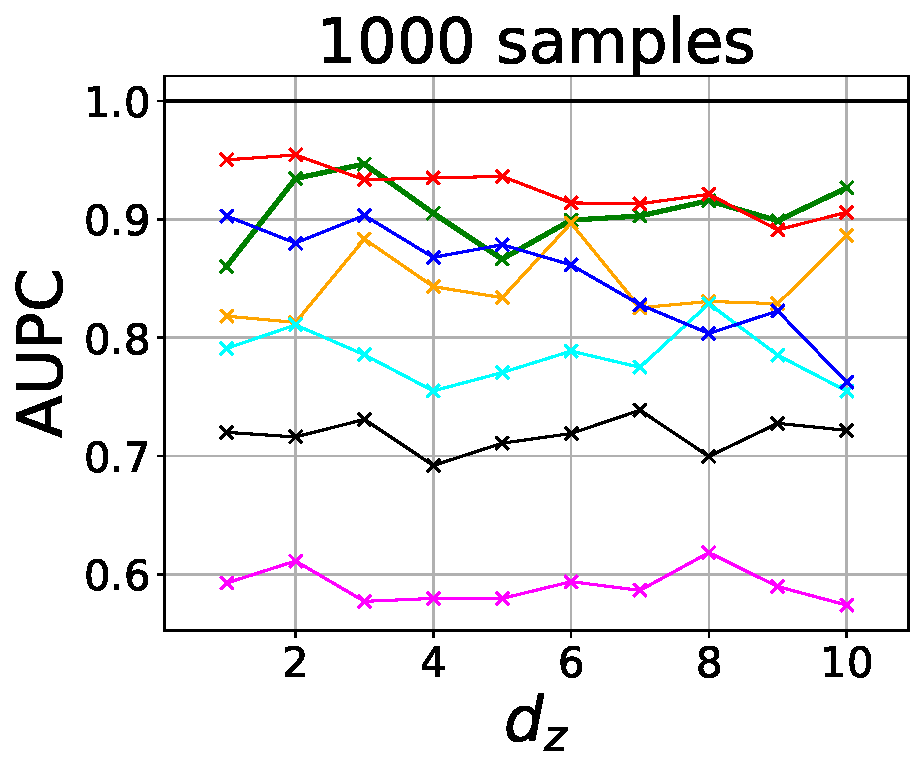
\includegraphics[height=2.2cm]{sections/appendix/independence_testing_kernel/new_figures/nsamples_fixed_1000_strobl_dim_1_10_aupc.pdf} & 
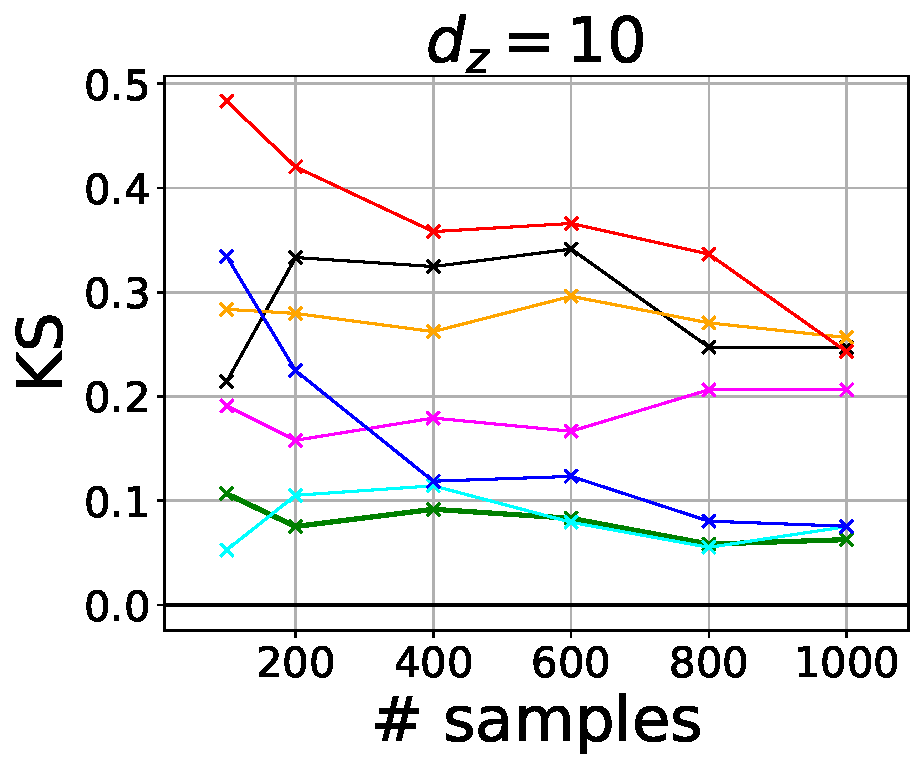
\includegraphics[height=2.2cm]{sections/appendix/independence_testing_kernel/new_figures/dim_fixed_10_strobl_ks.pdf}& 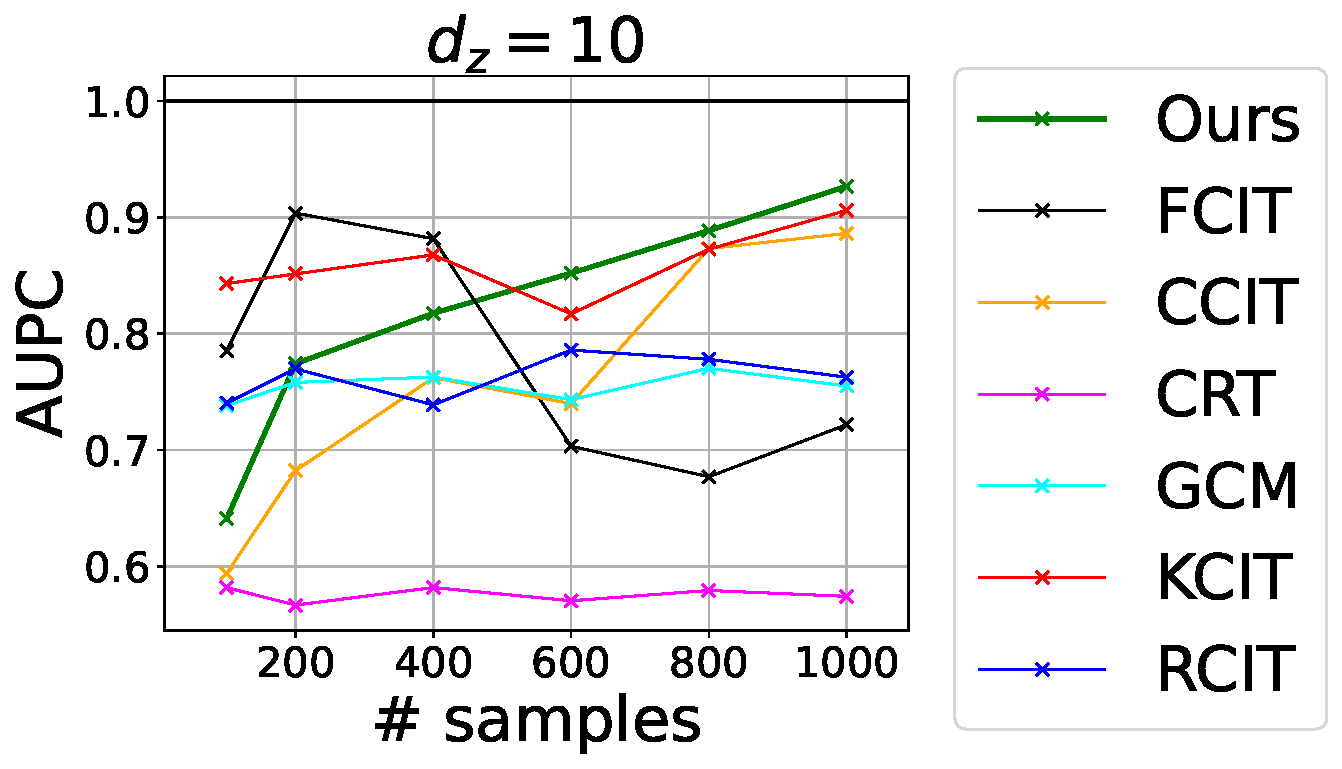
\includegraphics[height=2.2cm]{sections/appendix/independence_testing_kernel/new_figures/dim_fixed_10_strobl_aupc.pdf} 
\end{tabular}
\caption{Comparison of the KS statistic (lower is better) and the AUPC (higher is better) of our testing procedure with other SoTA tests on the two problems presented in~\eqref{exp-strobl-h0} and~\eqref{exp-strobl-h1}  with Gaussian noises. Each point in the figures is obtained by repeating the experiment forx 100 independent trials. (\emph{Left, middle-left}): the KS and AUPC obtained by each test when varying the dimension $d_z$ from 1 to 10, while fixing the number of samples $n$ to $1000$. (\emph{Middle-right, right}): the KS and AUPC obtained by each test when varying the number of samples $n$ from 100 to 1000, while fixing the dimension $d_z$ to $10$. 
\label{fig-exp-strobl-ks-supp}}
\vspace{-0.5cm}
\end{figure*}




\begin{figure*}[h]
\begin{tabular}{cccc} 
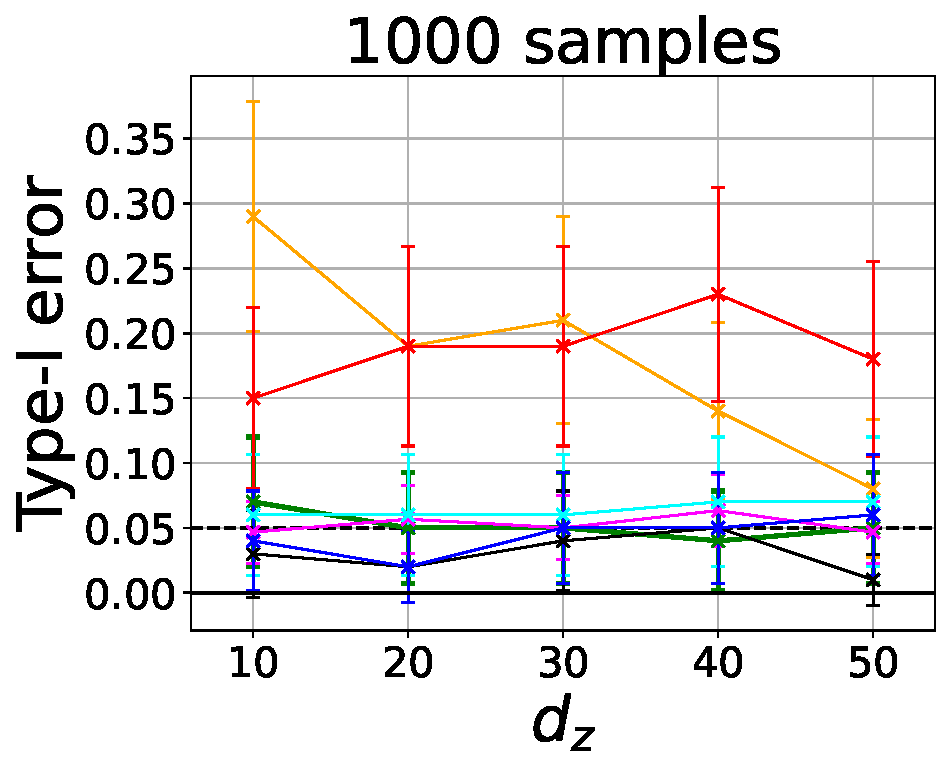
\includegraphics[height=2.2cm]{sections/appendix/independence_testing_kernel/figures_strobl_highdim_gaussian/nsamples_fixed_1000_strobl_dim_10_50_typeI.pdf}& 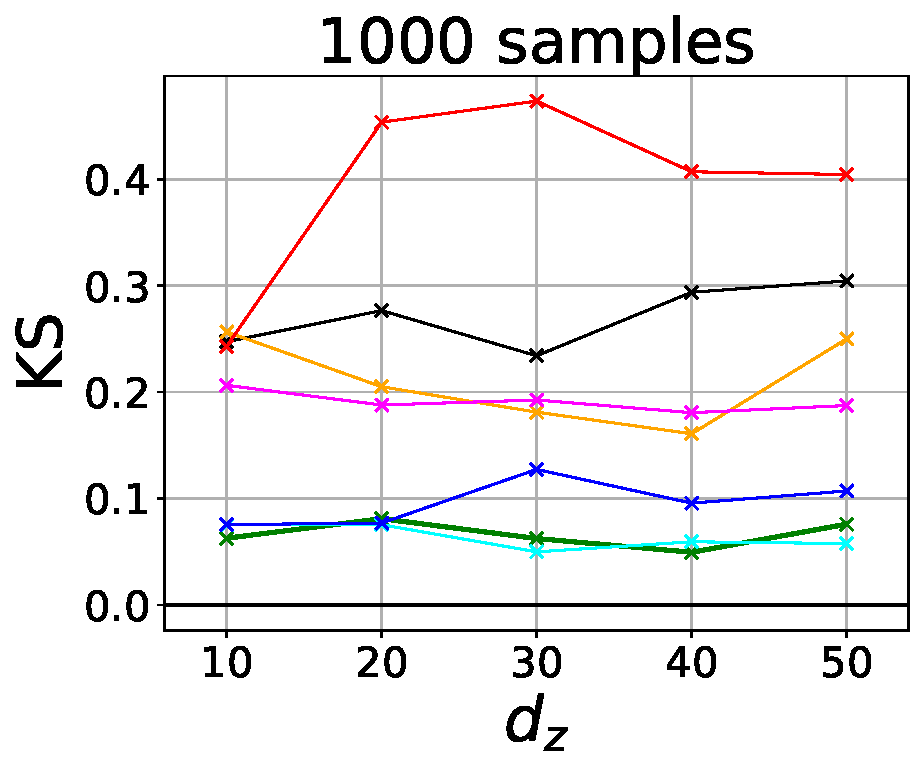
\includegraphics[height=2.2cm]{sections/appendix/independence_testing_kernel/figures_strobl_highdim_gaussian/nsamples_fixed_1000_strobl_dim_10_50_ks.pdf} & 
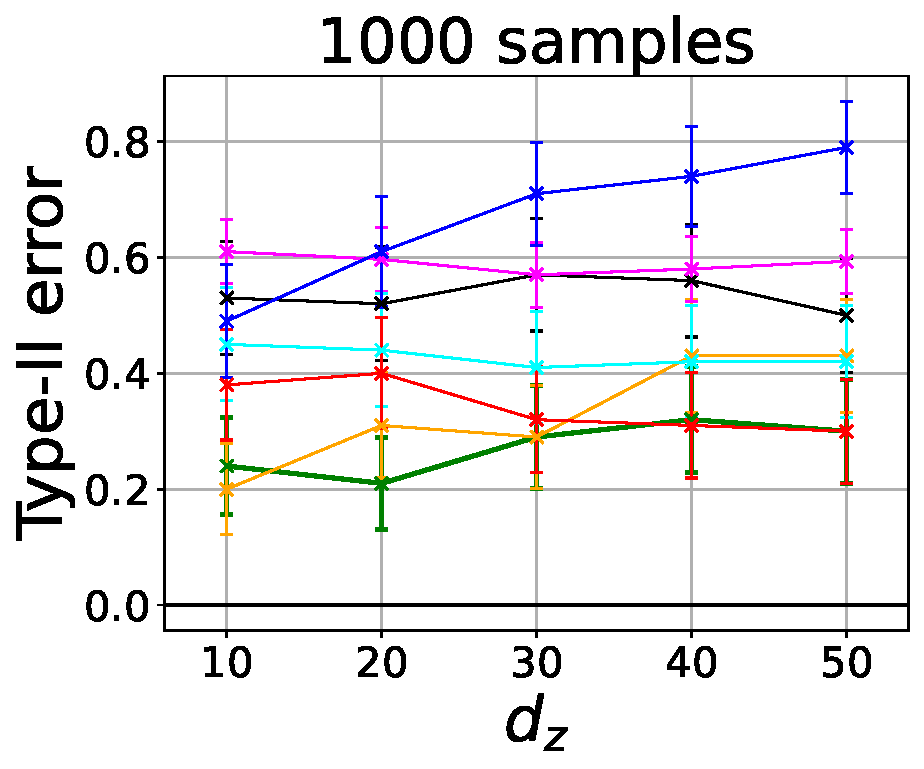
\includegraphics[height=2.2cm]{sections/appendix/independence_testing_kernel/figures_strobl_highdim_gaussian/nsamples_fixed_1000_strobl_dim_10_50_typeII.pdf}& 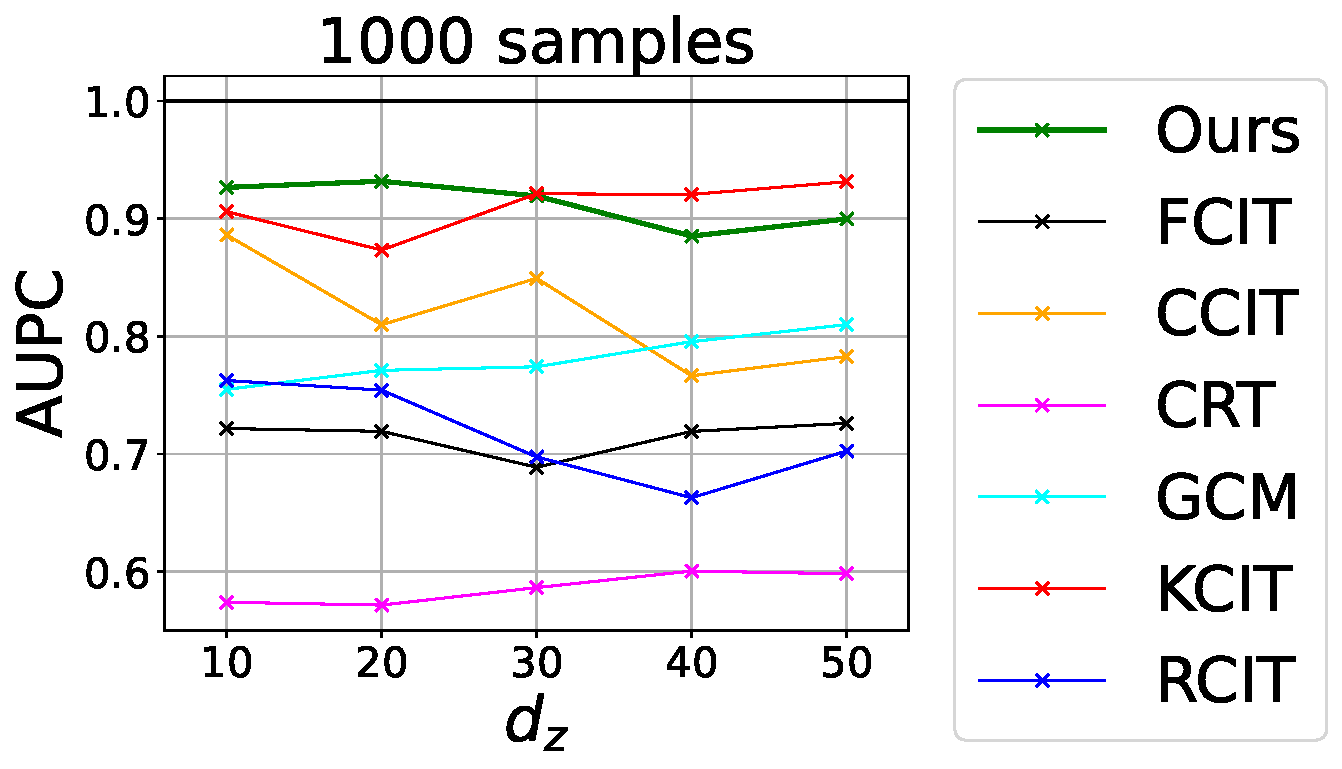
\includegraphics[height=2.2cm]{sections/appendix/independence_testing_kernel/figures_strobl_highdim_gaussian/nsamples_fixed_1000_strobl_dim_10_50_aupc.pdf}
\end{tabular}
\caption{Comparison of the type-I error at level $\alpha=0.05$ (dashed line), type-II error (lower is better), KS statistic and the AUPC of our testing procedure with other SoTA tests on the two problems presented in Eq.~\eqref{exp-strobl-h0} and Eq.~\eqref{exp-strobl-h1} with Gaussian noises. Each point in the figures is obtained by repeating the experiment for 100 independent trials. In each plot the dimension $d_z$ is varying from 10 to 50; here, the number of samples $n$ is fixed and equals to $1000$. 
\label{fig-exp-strobl-highdim-gaussian-supp}}
\vspace{-0.6cm}
\end{figure*}











\newpage


\subsubsection{Laplace Case}
\vspace{-0.4cm}






\begin{figure*}[htb]
\begin{tabular}{cccc} 
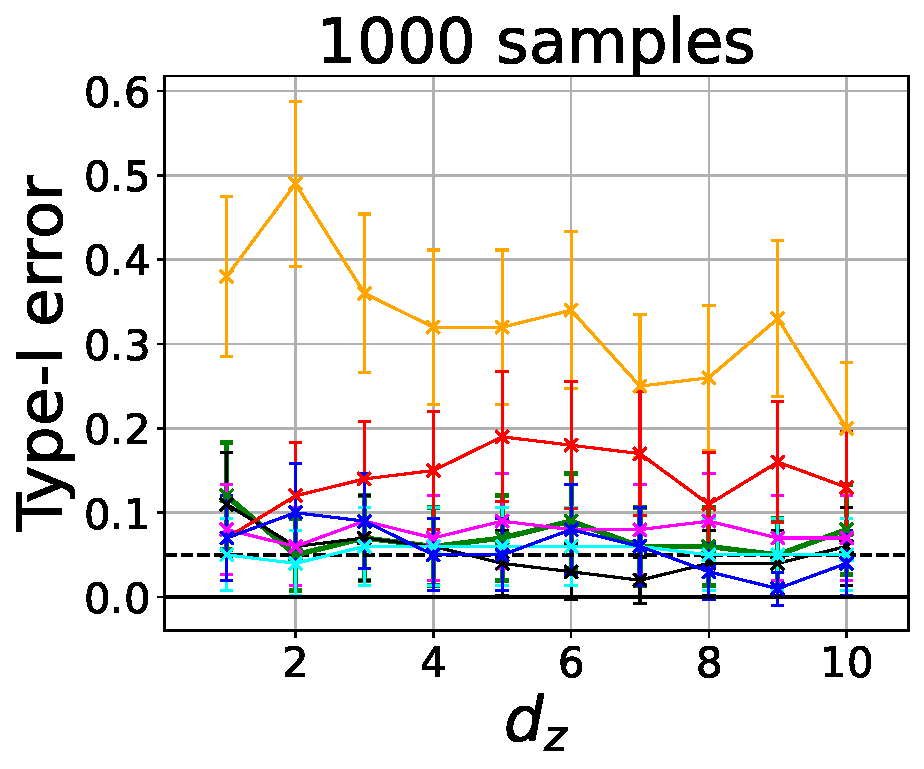
\includegraphics[height=2.2cm]{sections/appendix/independence_testing_kernel/new_figures_lap/nsamples_fixed_1000_strobl_dim_1_10_typeI.pdf}& 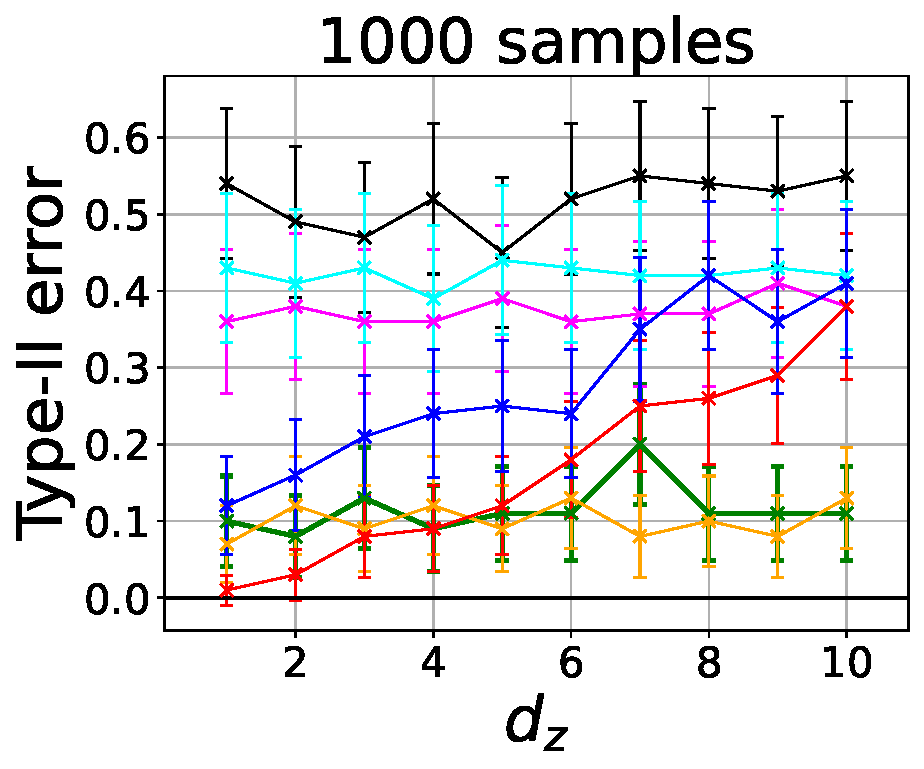
\includegraphics[height=2.2cm]{sections/appendix/independence_testing_kernel/new_figures_lap/nsamples_fixed_1000_strobl_dim_1_10_typeII.pdf} & 
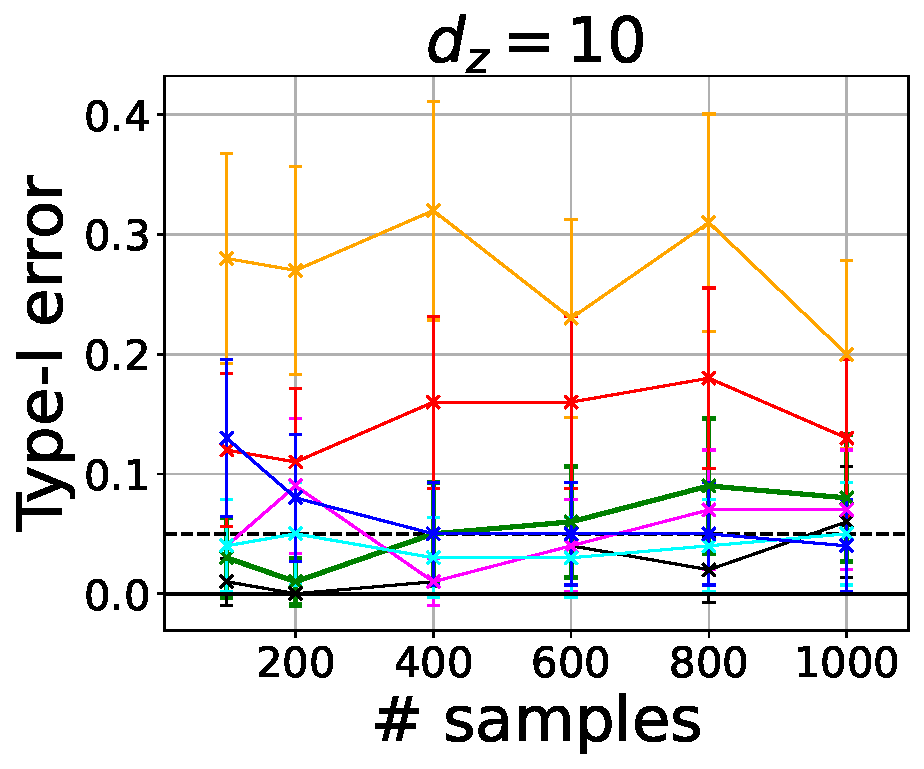
\includegraphics[height=2.2cm]{sections/appendix/independence_testing_kernel/new_figures_lap/dim_fixed_10_strobl_typeI.pdf}& 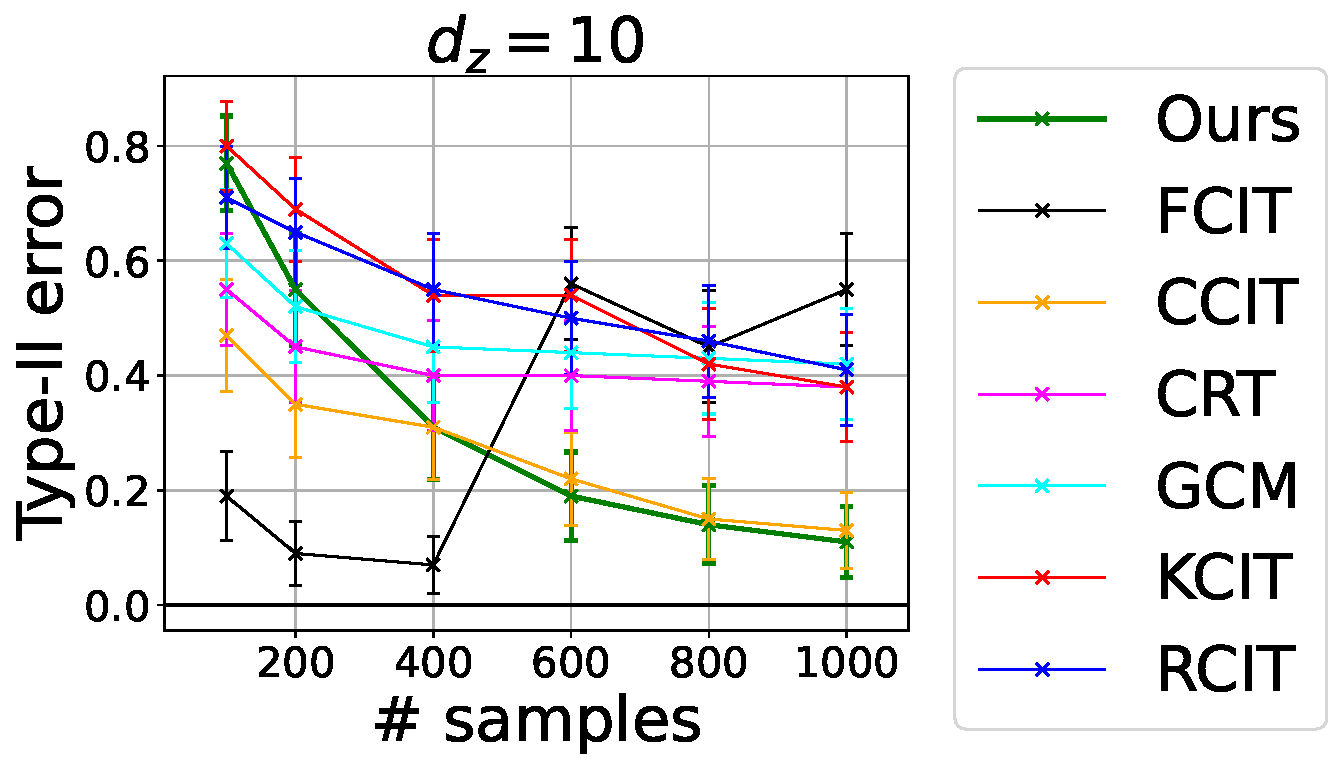
\includegraphics[height=2.2cm]{sections/appendix/independence_testing_kernel/new_figures_lap/dim_fixed_10_strobl_typeII.pdf} 
\end{tabular}
\caption{Comparison of the type-I error at level $\alpha=0.05$ (dashed line) and the type-II error (lower is better) of our test procedure with other SoTA tests on the two problems presented in~\eqref{exp-strobl-h0} and~\eqref{exp-strobl-h1} with Laplace noises. Each point in the figures is obtained by repeating the experiment for 100 independent trials. (\emph{Left, middle-left}): type-I and type-II errors obtained by each test when varying the dimension $d_z$ from 1 to 10; here, the number of samples $n$ is fixed and equals to $1000$. (\emph{Middle-right, right}): type-I and type-II errors obtained by each test when varying the number of samples $n$ from 100 to 1000; here, the dimension $d_z$ is fixed and equals to $10$.
\label{fig-exp-strobl-laplace-supp}}
\vspace{-0.5cm}
\end{figure*}




\begin{figure*}[htb]
\begin{tabular}{cccc} 
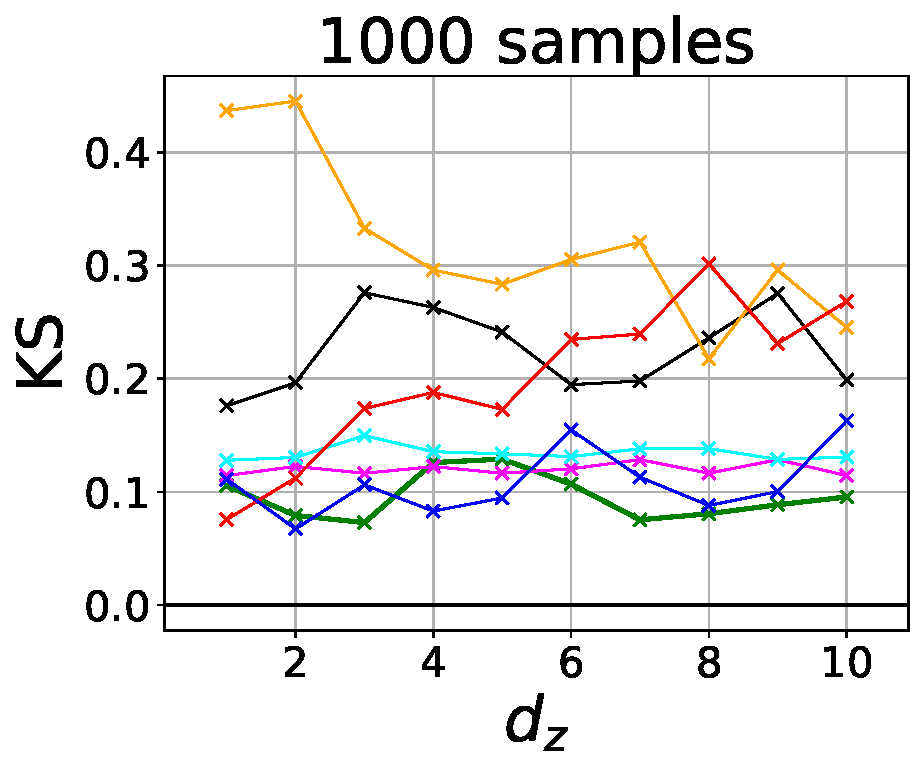
\includegraphics[height=2.2cm]{sections/appendix/independence_testing_kernel/new_figures_lap/nsamples_fixed_1000_strobl_dim_1_10_ks.pdf}& 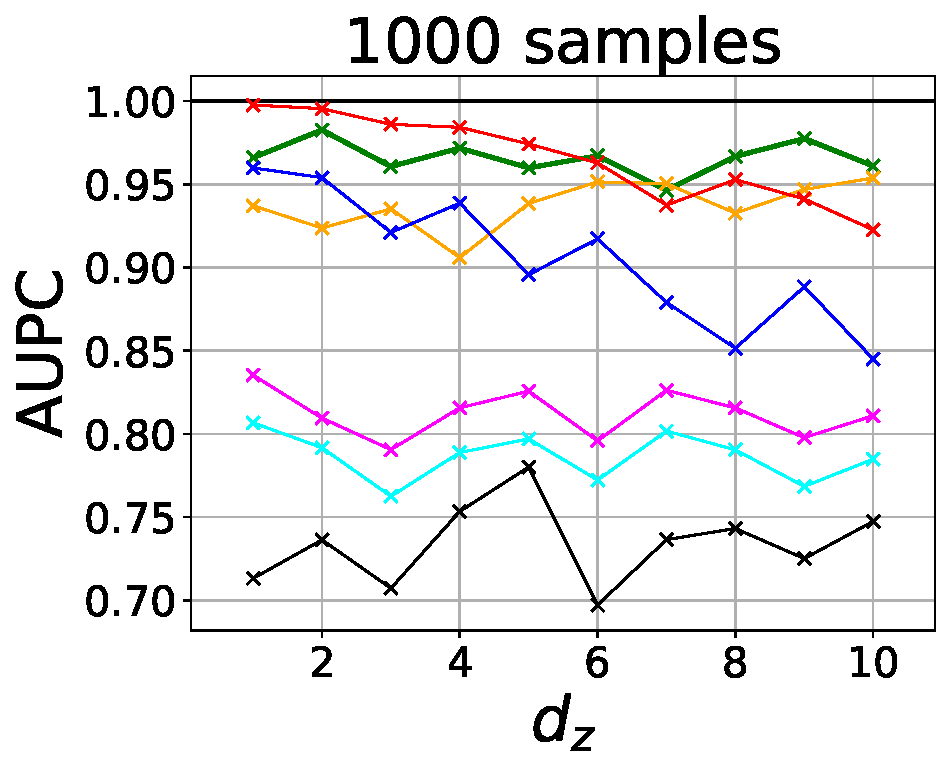
\includegraphics[height=2.2cm]{sections/appendix/independence_testing_kernel/new_figures_lap/nsamples_fixed_1000_strobl_dim_1_10_aupc.pdf} & 
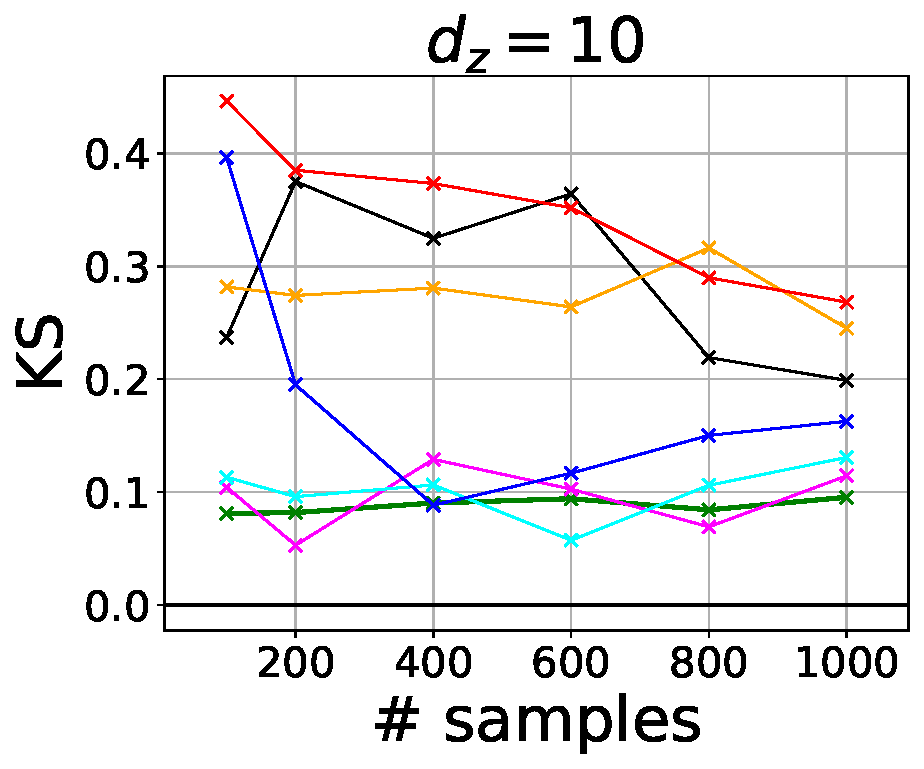
\includegraphics[height=2.2cm]{sections/appendix/independence_testing_kernel/new_figures_lap/dim_fixed_10_strobl_ks.pdf}& 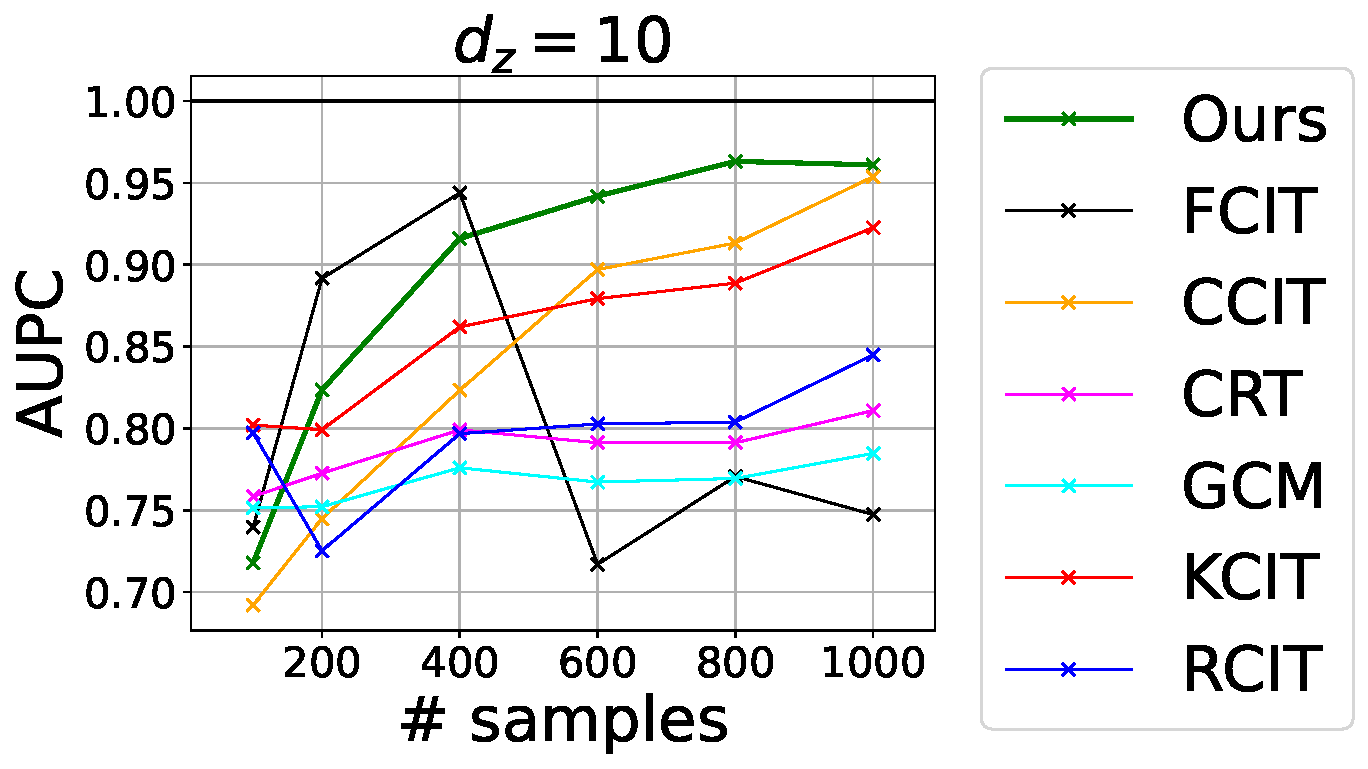
\includegraphics[height=2.2cm]{sections/appendix/independence_testing_kernel/new_figures_lap/dim_fixed_10_strobl_aupc.pdf} 
\end{tabular}
\caption{Comparison of the KS statistic and the AUPC of our testing procedure with other SoTA tests on the two problems presented in Eq.~\eqref{exp-strobl-h0} and Eq.~\eqref{exp-strobl-h1}  with Laplace noises. Each point in the figures is obtained by repeating the experiment for 100 independent trials. (\emph{Left, middle-left}): the KS statistic and AUPC (respectively) obtained by each test when varying the dimension $d_z$ from 1 to 10; here, the number of samples $n$ is fixed and equals to $1000$. (\emph{Middle-right, right}): the KS and AUPC (respectively), obtained by each test when varying the number of samples $n$ from 100 to 1000; here, the dimension $d_z$ is fixed and equals to $10$.
\label{fig-exp-strobl-ks-laplace-supp}}
\vspace{-0.5cm}
\end{figure*}


\begin{figure*}[ht]
\begin{tabular}{cccc} 
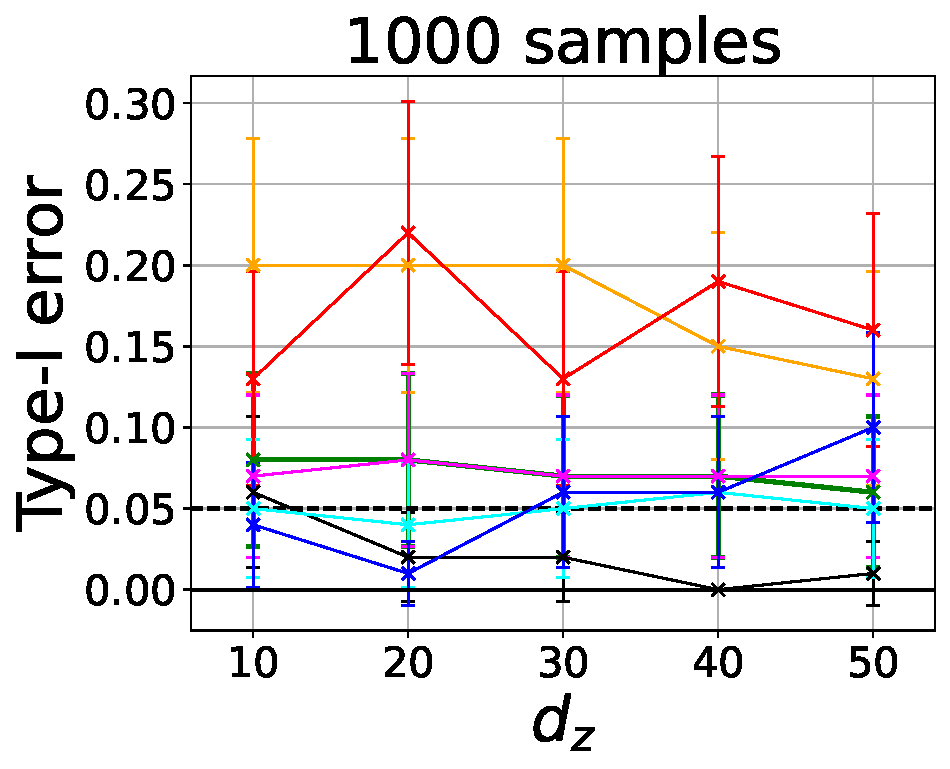
\includegraphics[height=2.2cm]{sections/appendix/independence_testing_kernel/figures_strobl_highdim_lap/nsamples_fixed_1000_strobl_dim_10_50_typeI.pdf}& 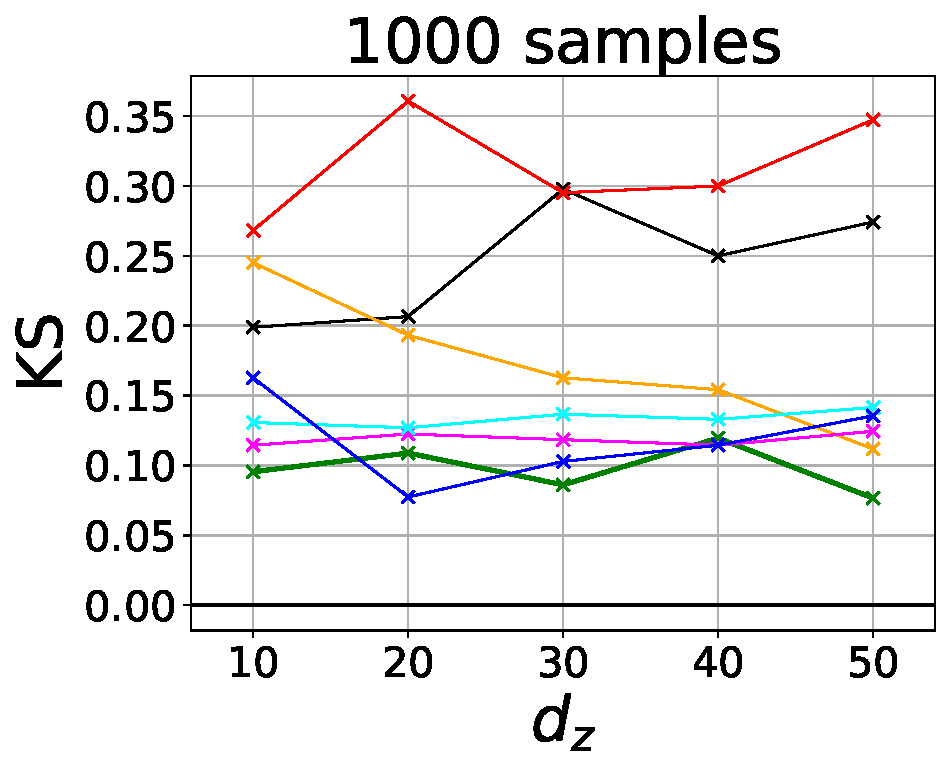
\includegraphics[height=2.2cm]{sections/appendix/independence_testing_kernel/figures_strobl_highdim_lap/nsamples_fixed_1000_strobl_dim_10_50_ks.pdf} & 
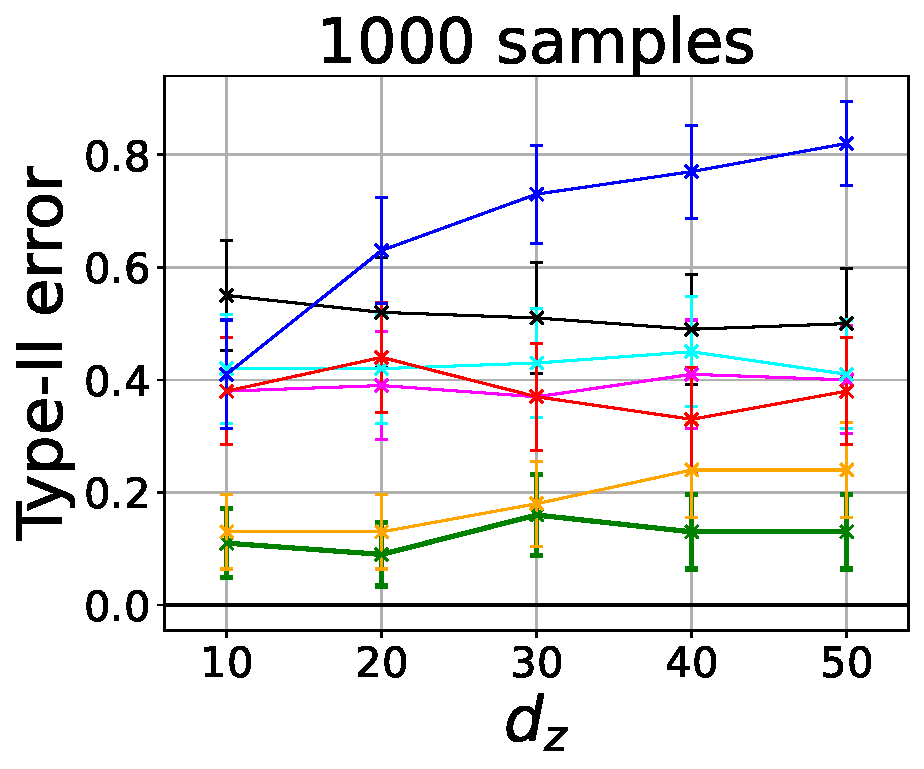
\includegraphics[height=2.2cm]{sections/appendix/independence_testing_kernel/figures_strobl_highdim_lap/nsamples_fixed_1000_strobl_dim_10_50_typeII.pdf}& 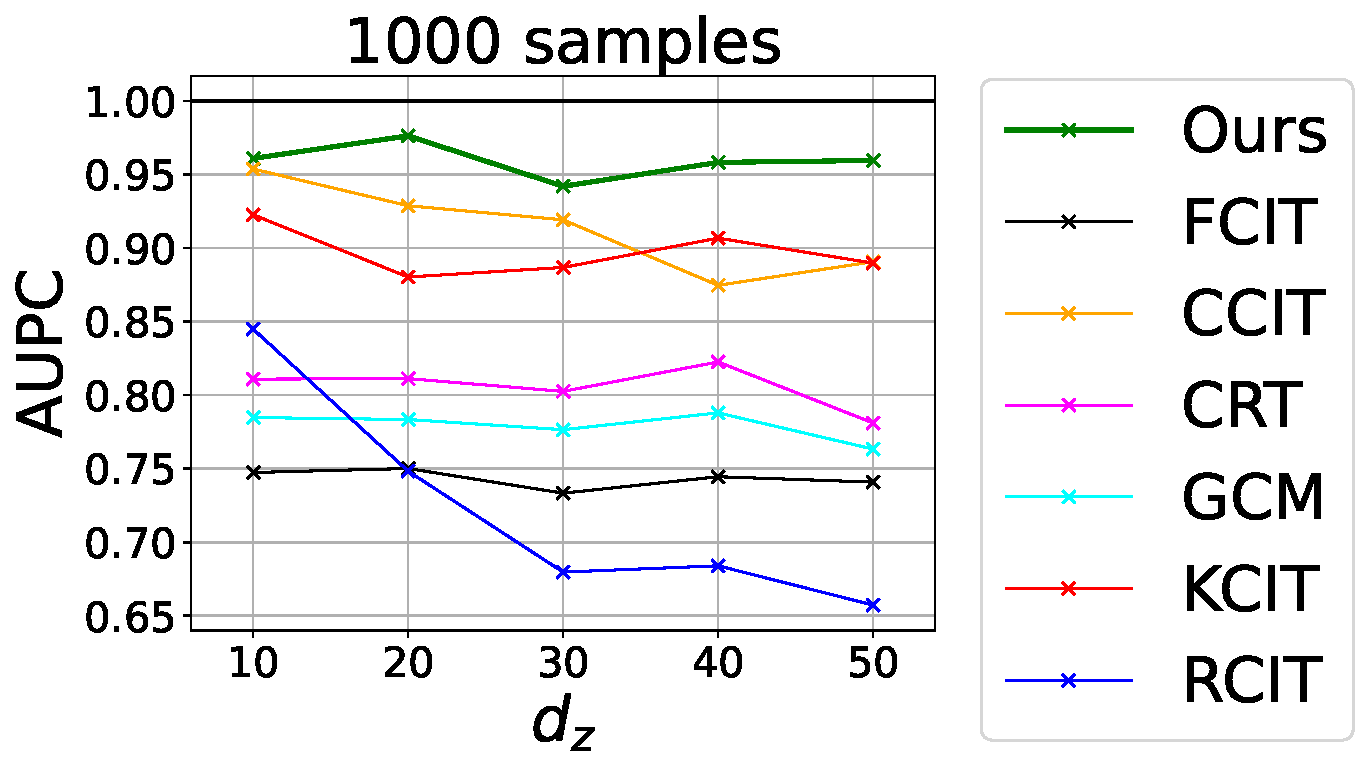
\includegraphics[height=2.2cm]{sections/appendix/independence_testing_kernel/figures_strobl_highdim_lap/nsamples_fixed_1000_strobl_dim_10_50_aupc.pdf}
\end{tabular}
\caption{Comparison of the type-I error at level $\alpha=0.05$ (dashed line), type-II error (lower is better), KS statistic and the AUPC of our testing procedure with other SoTA tests on the two problems presented in Eq.~\eqref{exp-strobl-h0} and Eq.~\eqref{exp-strobl-h1} with Laplace noises. Each point in the figures is obtained by repeating the experiment for 100 independent trials. In each plot the dimension $d_z$ is varying from 10 to 50; here, the number of samples $n$ is fixed and equals to $1000$.
\label{fig-exp-strobl-highdim-laplace-supp}}
\vspace{-0.8cm}
\end{figure*}


\newpage
\subsection{Additional experiments on Problems~\eqref{li-exp-h0} and~\eqref{li-exp-h1}}
\label{sec-exp-li}
\vspace{-0.2cm}
\subsubsection{Gaussian Case}
\vspace{-0.4cm}


% Figure~\ref{fig-exp-li-ks-gauss} compares the KS statistic and the AUPC obtained by different testing procedures in the exact same setting considered in Figure~\ref{fig-exp-li}. Following that figure, one can see that our method outperforms the other tests both in terms of type-I error and power. In addition, Figure~\ref{fig-exp-li-ks-highdim} presets the results obtained in a high dimensional regime, showing that our method tends to outperform the existing tests in most cases.


\begin{figure*}[htb]
\begin{tabular}{cccc} 
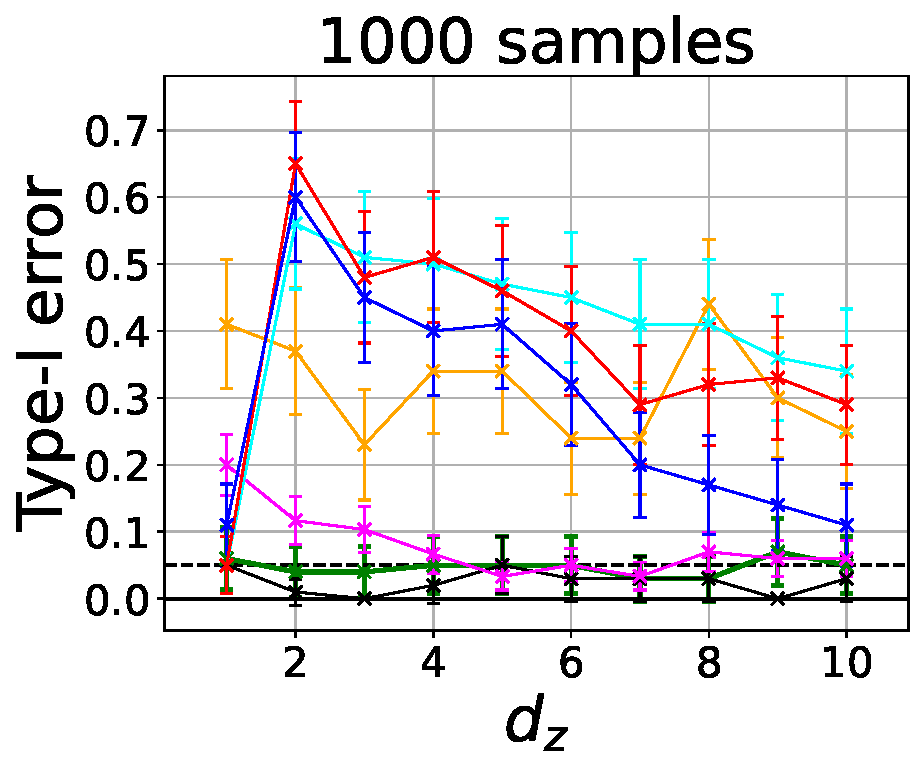
\includegraphics[height=2.2cm]{sections/appendix/independence_testing_kernel/new_figures/nsamples_fixed_1000_li_dim_1_10_typeI.pdf}& 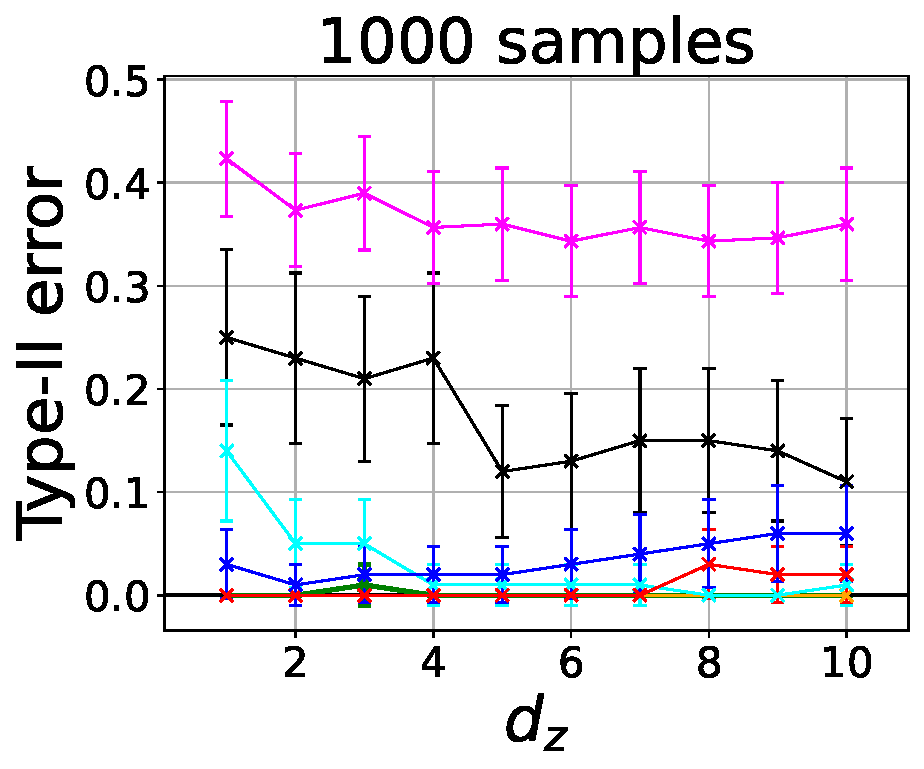
\includegraphics[height=2.2cm]{sections/appendix/independence_testing_kernel/new_figures/nsamples_fixed_1000_li_dim_1_10_typeII.pdf} & 
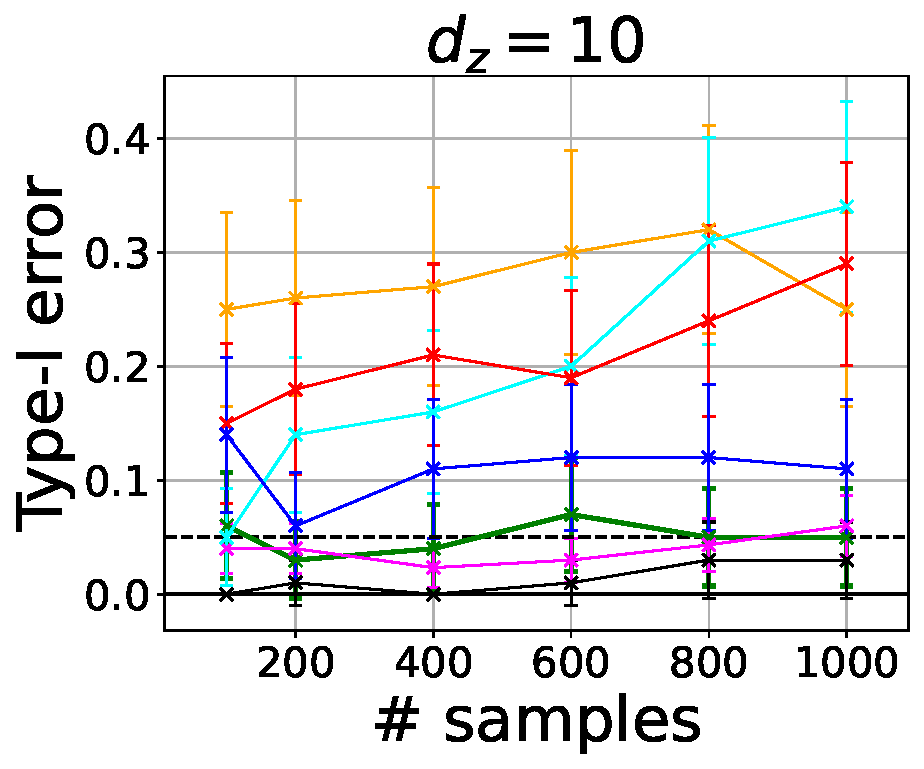
\includegraphics[height=2.2cm]{sections/appendix/independence_testing_kernel/new_figures/dim_fixed_10_li_typeI.pdf}& 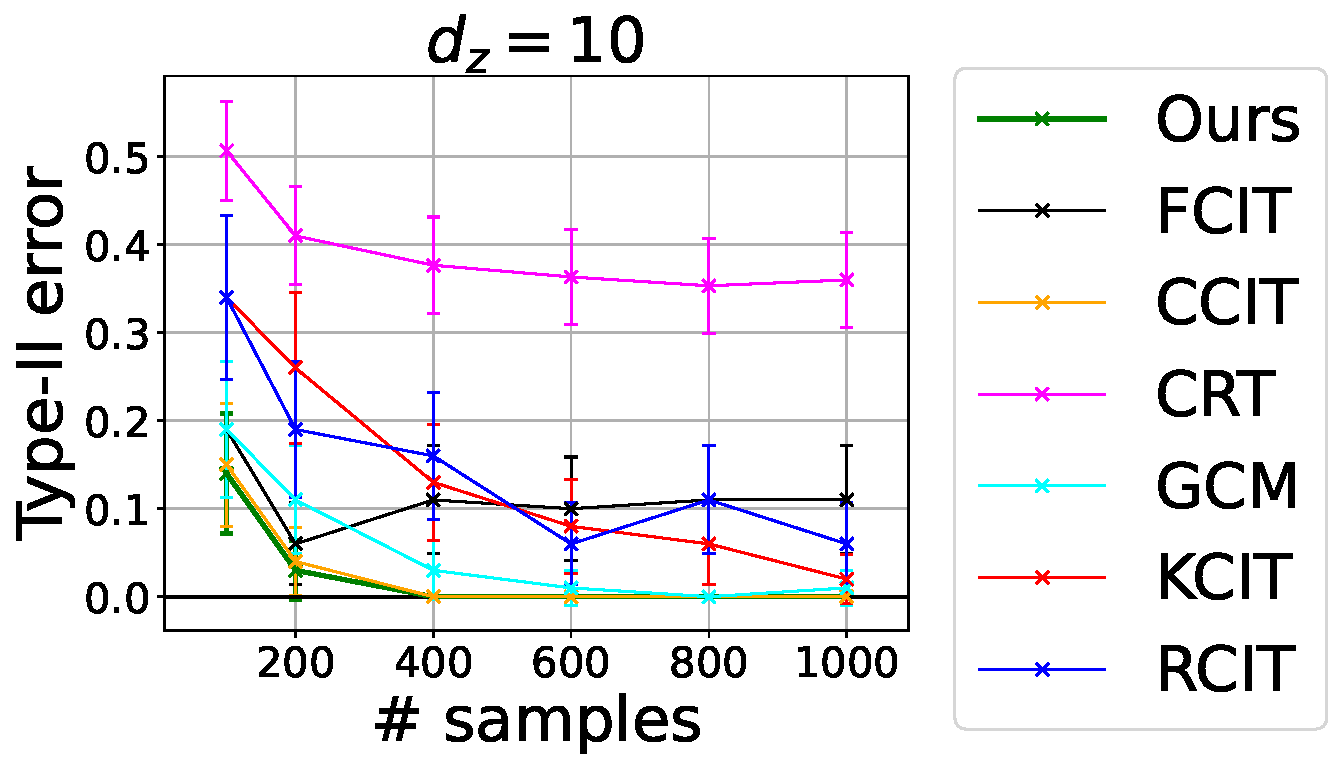
\includegraphics[height=2.2cm]{sections/appendix/independence_testing_kernel/new_figures/dim_fixed_10_li_typeII.pdf} 
\end{tabular}
\caption{Comparison of the type-I error at level $\alpha=0.05$ (dashed line) and the type-II error (lower is better) of our test procedure with other SoTA tests on the two problems presented in~\eqref{li-exp-h0} and~\eqref{li-exp-h1}  with Gaussian noises. Each point in the figures is obtained by repeating the experiment for 100 independent trials. (\emph{Left, middle-left}): type-I and type-II errors obtained by each test when varying the dimension $d_z$ from 1 to 10; here, the number of samples $n$ is fixed and equals to $1000$. (\emph{Middle-right, right}): type-I and type-II errors obtained by each test when varying the number of samples $n$ from 100 to 1000; here, the dimension $d_z$ is fixed and equals to $10$. 
\label{fig-exp-li-type-supp}}
\vspace{-0.5cm}
\end{figure*}


\begin{figure*}[ht]
\begin{tabular}{cccc} 
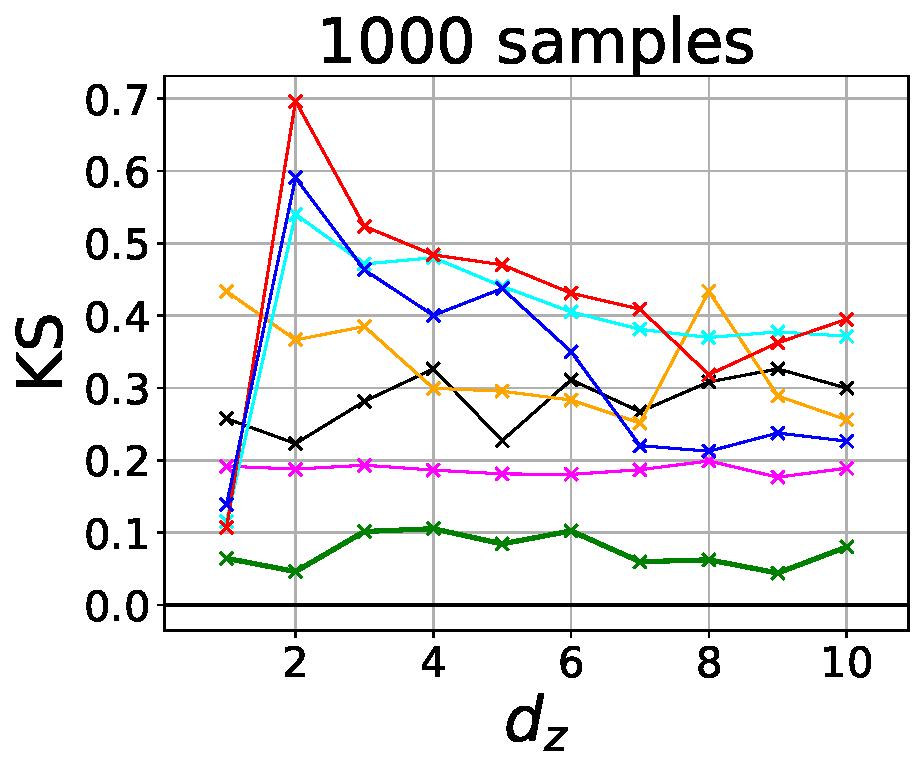
\includegraphics[height=2.2cm]{sections/appendix/independence_testing_kernel/figures_supp_mat/nsamples_fixed_1000_li_dim_1_10_ks.pdf}& 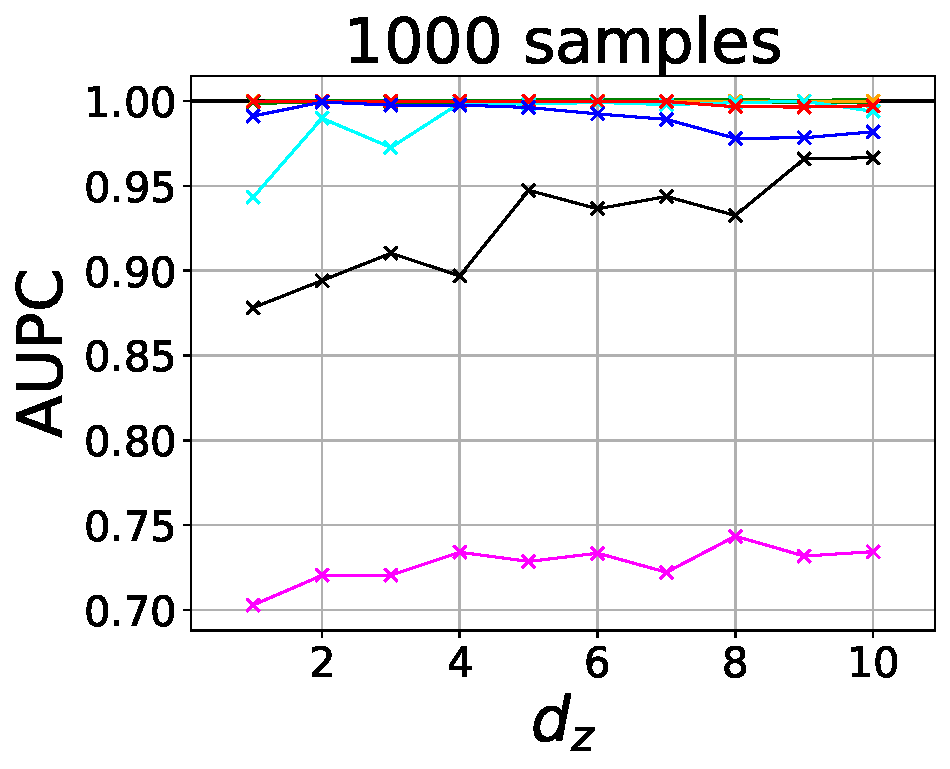
\includegraphics[height=2.2cm]{sections/appendix/independence_testing_kernel/figures_supp_mat/nsamples_fixed_1000_li_dim_1_10_aupc.pdf} & 
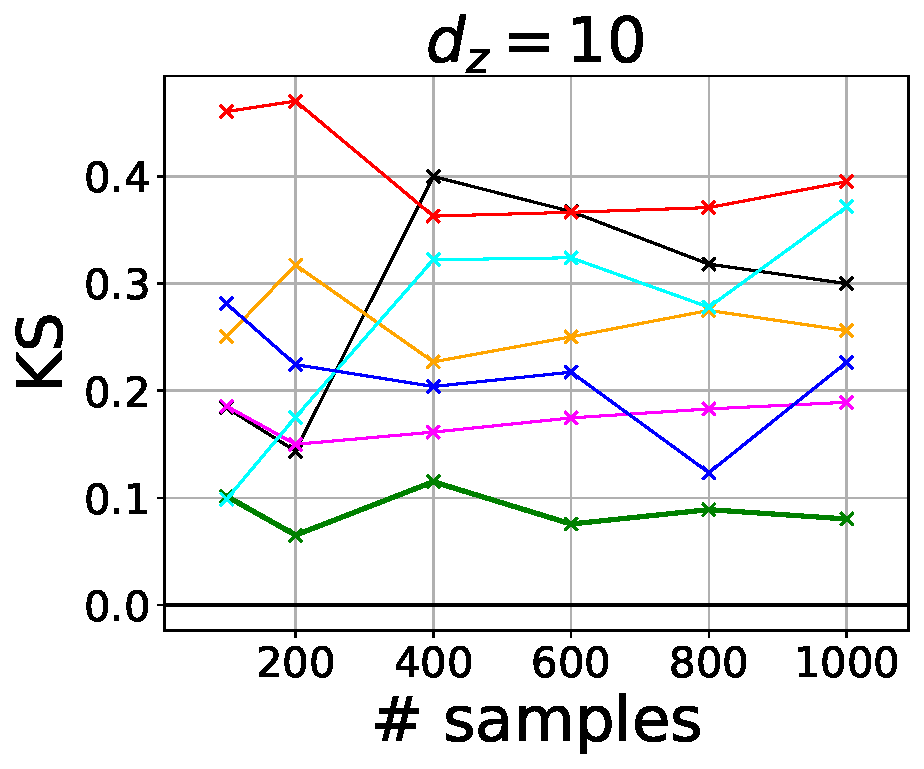
\includegraphics[height=2.2cm]{sections/appendix/independence_testing_kernel/figures_supp_mat/dim_fixed_10_li_ks.pdf}& 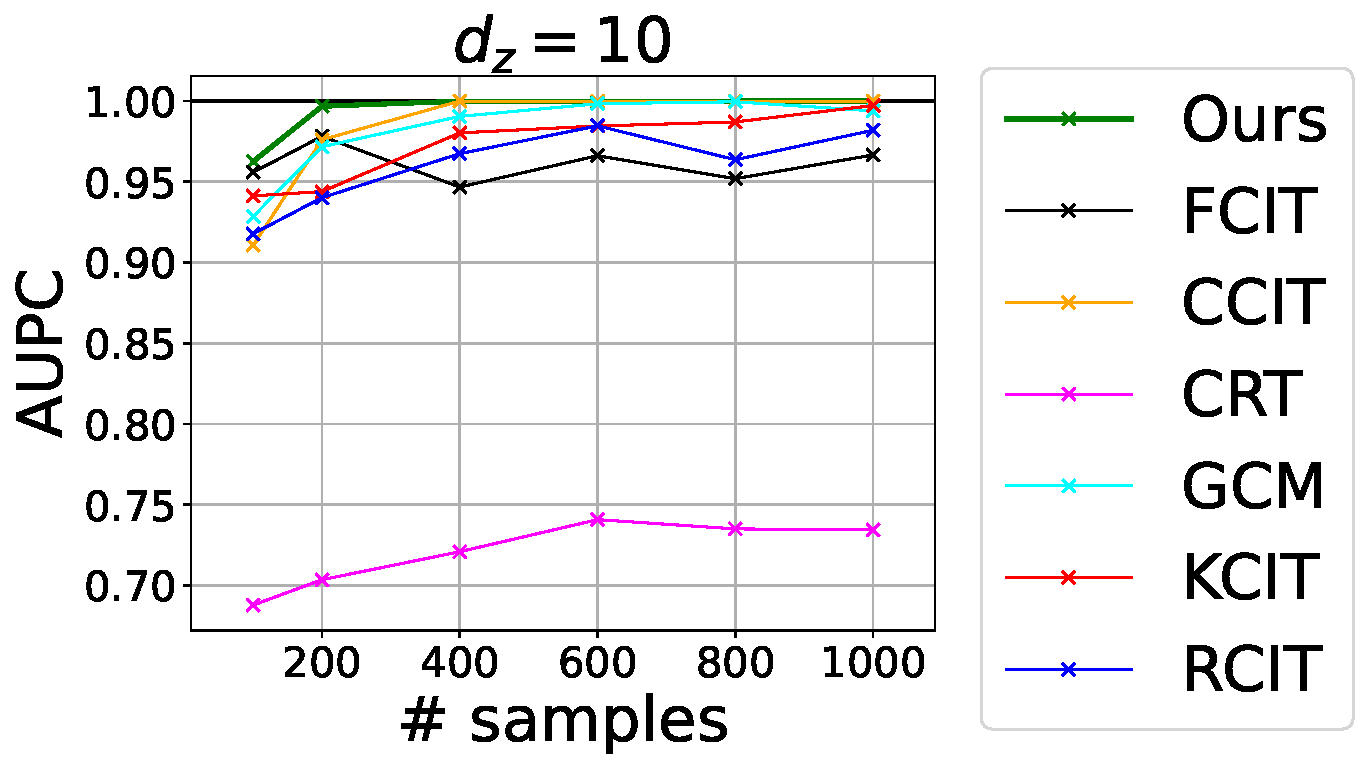
\includegraphics[height=2.2cm]{sections/appendix/independence_testing_kernel/figures_supp_mat/dim_fixed_10_li_aupc.pdf}
\end{tabular}
\caption{Comparison of the KS statistic and the AUPC of our testing procedure with other SoTA tests on the two problems presented in Eq.~\eqref{li-exp-h0} and Eq.~\eqref{li-exp-h1} with Gaussian noises. Each point in the figures is obtained by repeating the experiment for 100 independent trials. (\emph{Left, middle-left}): the KS statistic and AUPC (respectively) obtained by each test when varying the dimension $d_z$ from 1 to 10; here, the number of samples $n$ is fixed and equals to $1000$. (\emph{Middle-right, right}): the KS and AUPC (respectively), obtained by each test when varying the number of samples $n$ from 100 to 1000; the dimension $d_z$ is fixed and equals $10$.
\label{fig-exp-li-ks-gauss-supp}}
\vspace{-0.8cm}
\end{figure*}


\begin{figure*}[ht]
\begin{tabular}{cccc} 
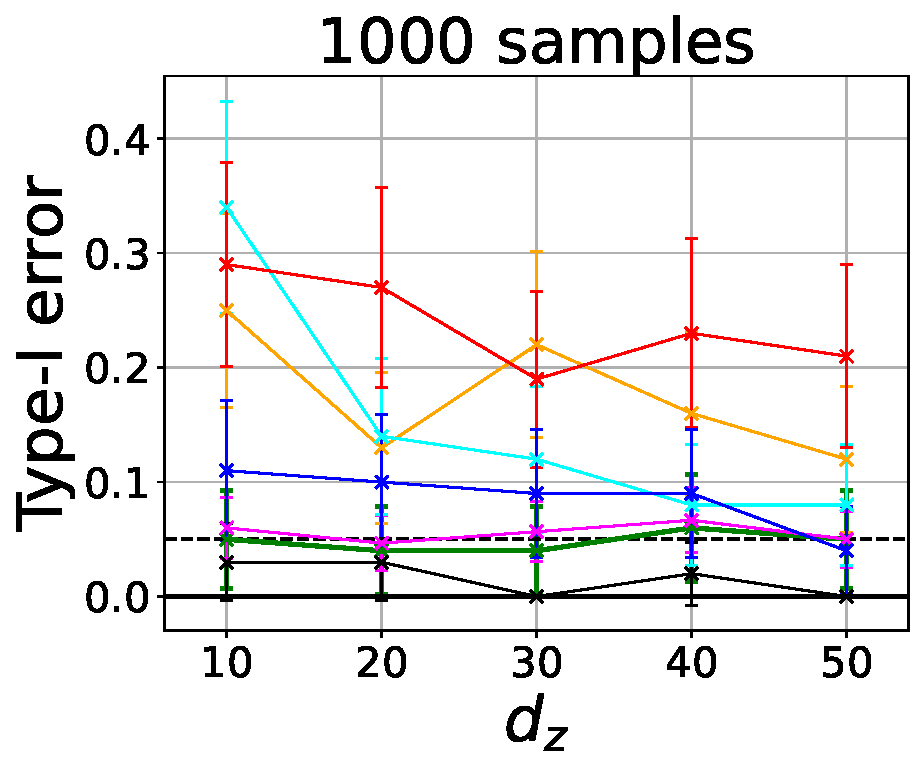
\includegraphics[height=2.2cm]{sections/appendix/independence_testing_kernel/figures_li_highdim/nsamples_fixed_1000_li_dim_10_50_typeI.pdf}& 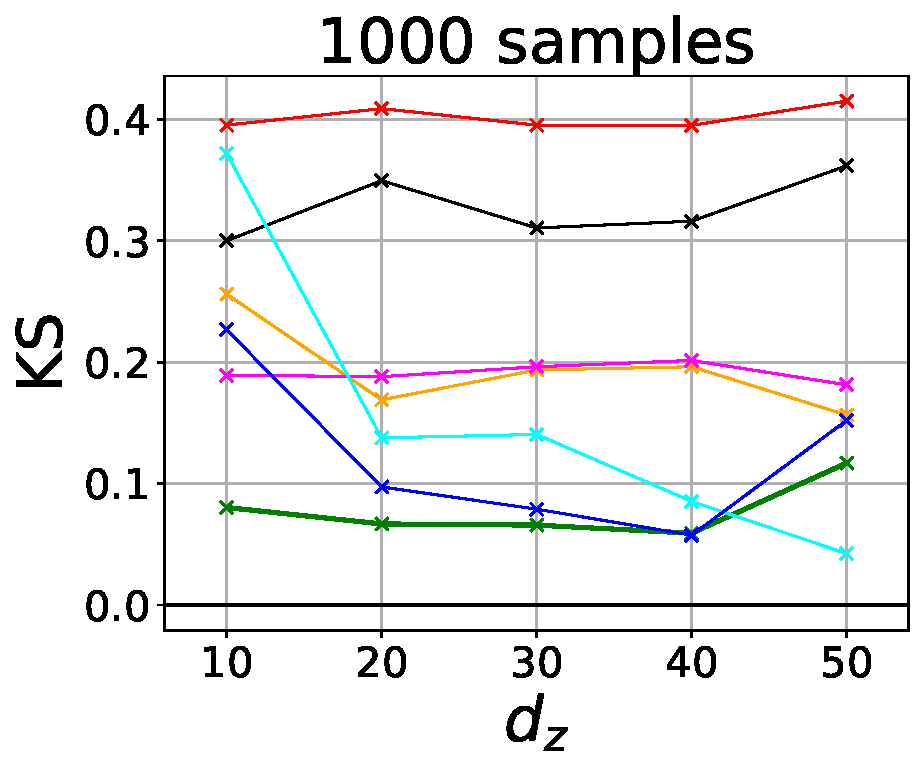
\includegraphics[height=2.2cm]{sections/appendix/independence_testing_kernel/figures_li_highdim/nsamples_fixed_1000_li_dim_10_50_ks.pdf} & 
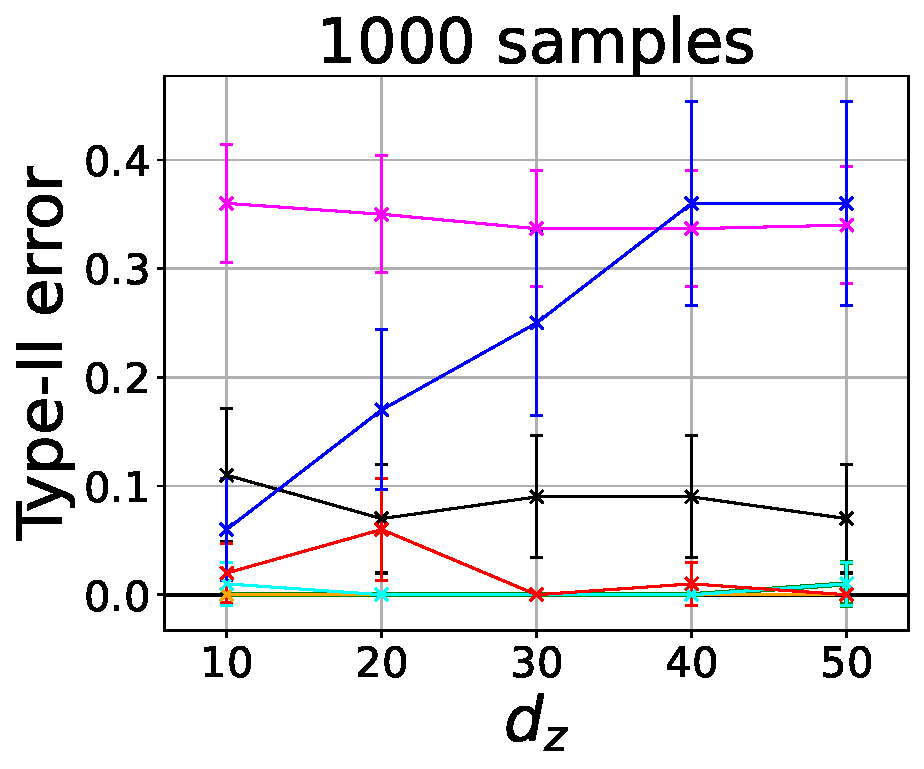
\includegraphics[height=2.2cm]{sections/appendix/independence_testing_kernel/figures_li_highdim/nsamples_fixed_1000_li_dim_10_50_typeII.pdf}& 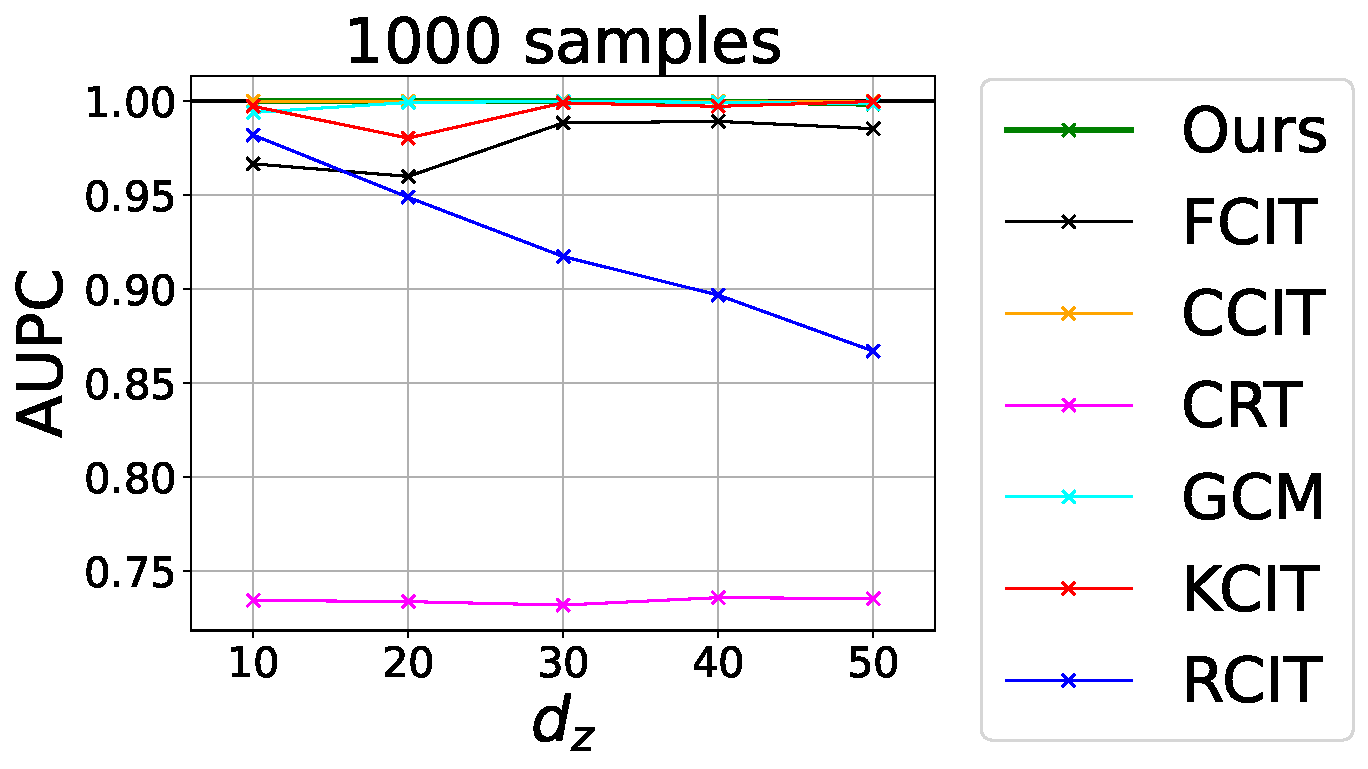
\includegraphics[height=2.2cm]{sections/appendix/independence_testing_kernel/figures_li_highdim/nsamples_fixed_1000_li_dim_10_50_aupc.pdf}
\end{tabular}
\caption{Comparison of the type-I error at level $\alpha=0.05$ (dashed line), type-II error (lower is better), KS statistic and the AUPC of our testing procedure with other SoTA tests on the two problems presented in Eq.~\eqref{li-exp-h0} and Eq.~\eqref{li-exp-h1} with Gaussian noises. Each point in the figures is obtained by repeating the experiment for 100 independent trials. In each plot the dimension $d_z$ is varying from 10 to 50; here, the number of samples $n$ is fixed and equals to $1000$. 
\label{fig-exp-li-highdim-gauss-supp}}
\vspace{-0.8cm}
\end{figure*}


\newpage
\subsubsection{Laplace Case}
\vspace{-0.4cm}
\begin{figure*}[h]
\begin{tabular}{cccc} 
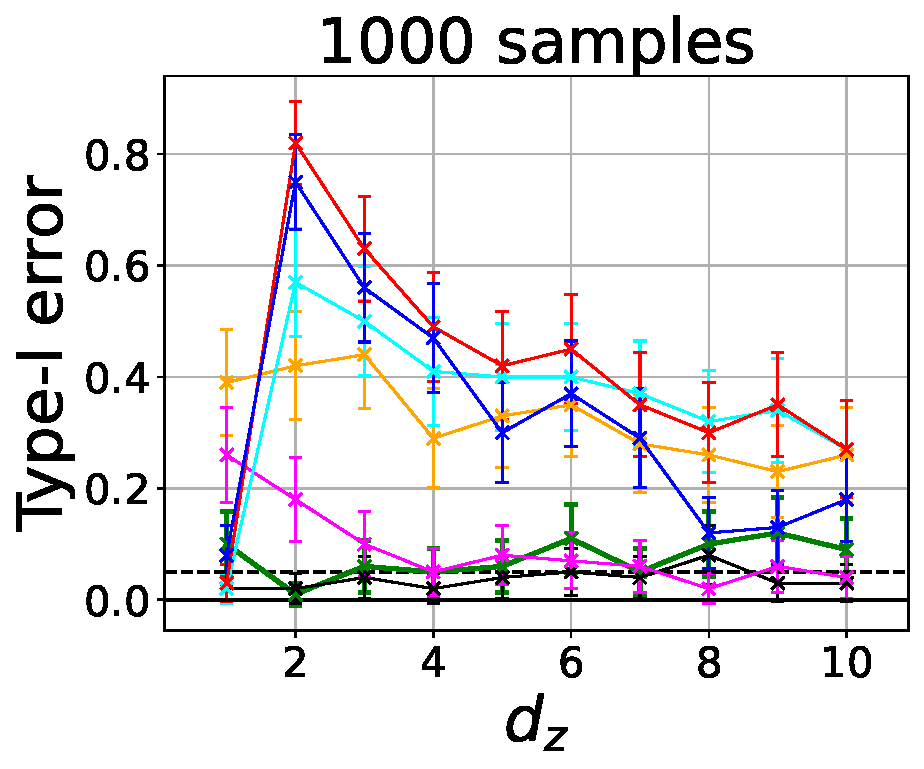
\includegraphics[height=2.2cm]{sections/appendix/independence_testing_kernel/new_figures_lap/nsamples_fixed_1000_li_dim_1_10_typeI.pdf}& 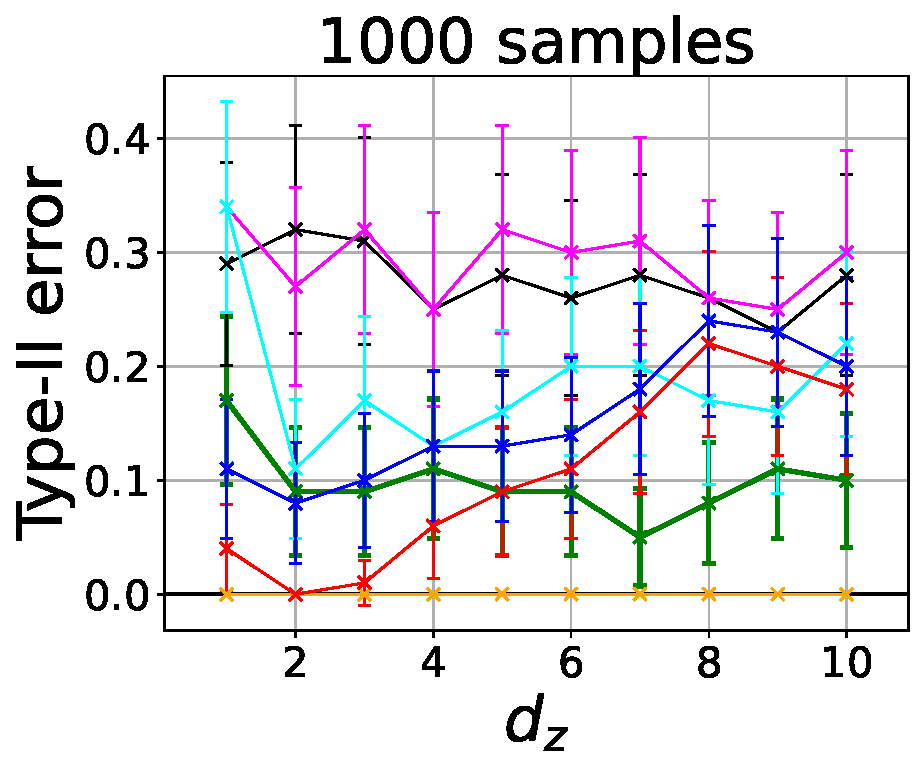
\includegraphics[height=2.2cm]{sections/appendix/independence_testing_kernel/new_figures_lap/nsamples_fixed_1000_li_dim_1_10_typeII.pdf} & 
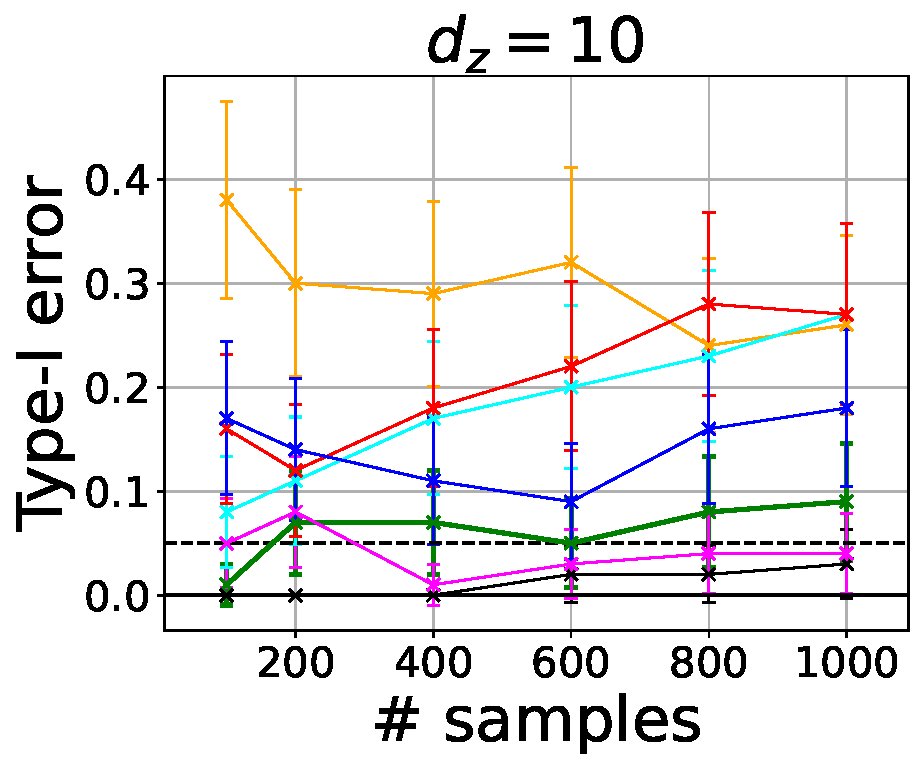
\includegraphics[height=2.2cm]{sections/appendix/independence_testing_kernel/new_figures_lap/dim_fixed_10_li_typeI.pdf}& 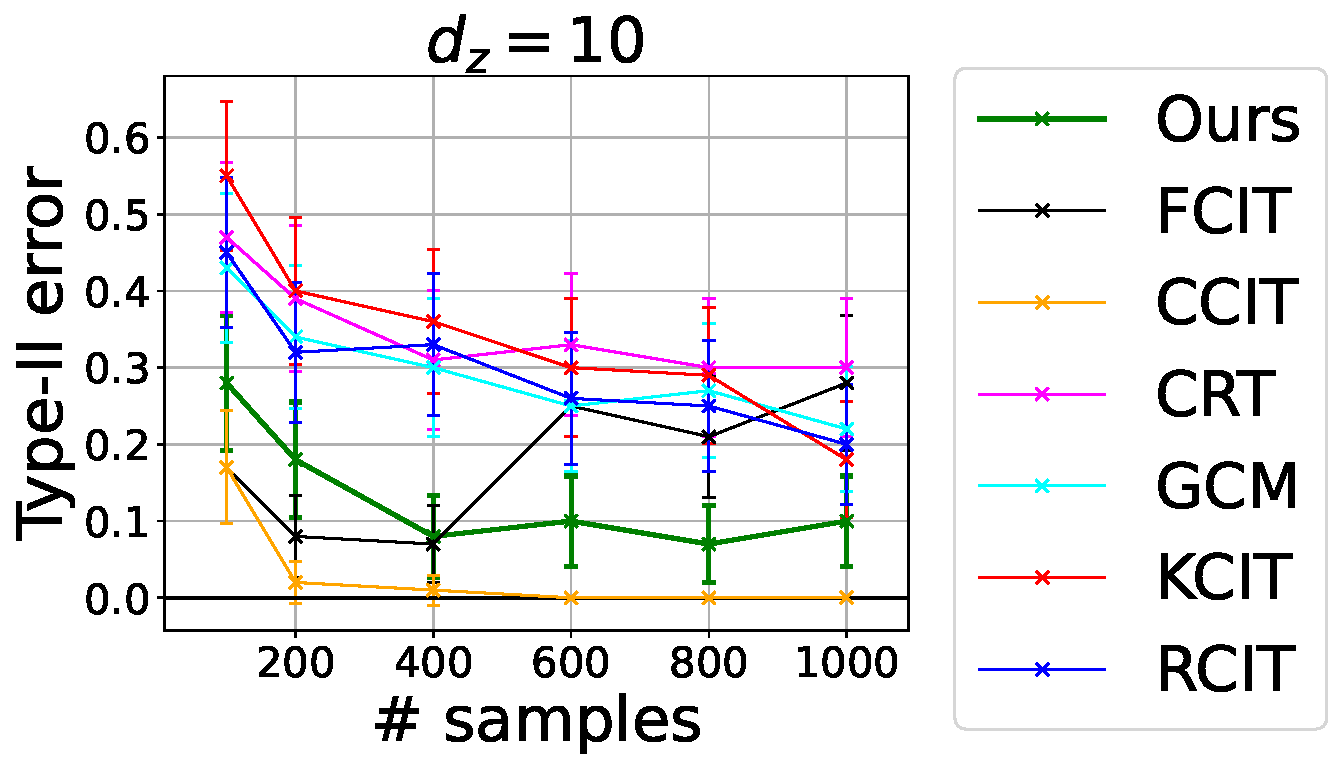
\includegraphics[height=2.2cm]{sections/appendix/independence_testing_kernel/new_figures_lap/dim_fixed_10_li_typeII.pdf} 
\end{tabular}
\caption{Comparison of the type-I error at level $\alpha=0.05$ (dashed line) and the type-II error (lower is better) of our test procedure with other SoTA tests on the two problems presented in~\eqref{li-exp-h0} and~\eqref{li-exp-h1}  with Laplace noises. Each point in the figures is obtained by repeating the experiment for 100 independent trials. (\emph{Left, middle-left}): type-I and type-II errors obtained by each test when varying the dimension $d_z$ from 1 to 10; here, the number of samples $n$ is fixed and equals to $1000$. (\emph{Middle-right, right}): type-I and type-II errors obtained by each test when varying the number of samples $n$ from 100 to 1000; the dimension $d_z$ is fixed and equals $10$. 
\label{fig-exp-li-laplace-supp}}
\vspace{-0.5cm}
\end{figure*}

\begin{figure*}[h]
\begin{tabular}{cccc} 
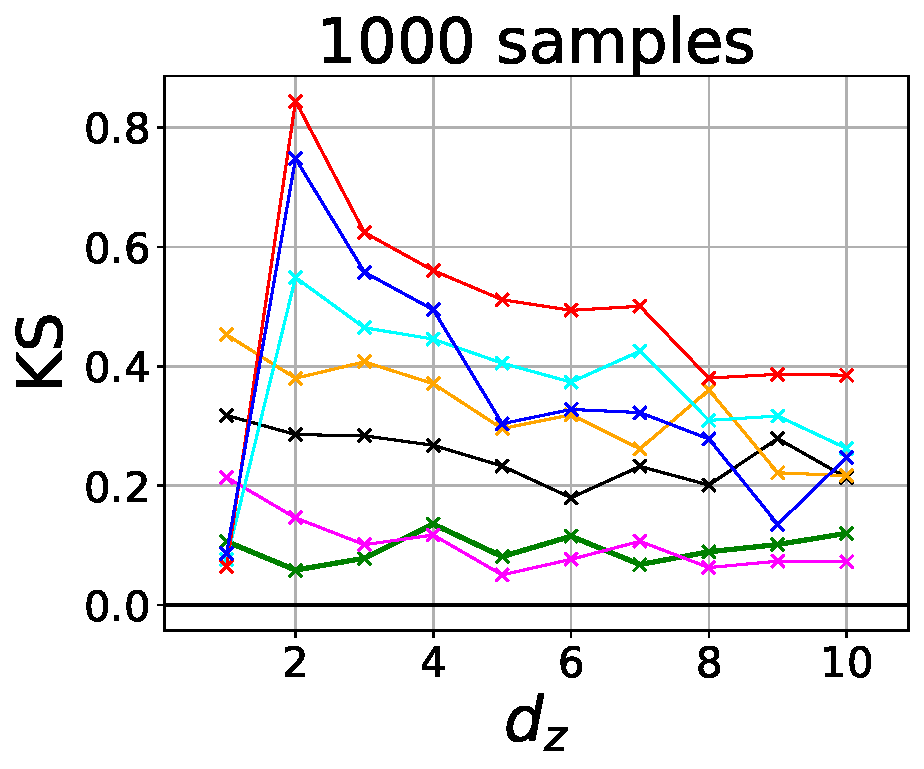
\includegraphics[height=2.2cm]{sections/appendix/independence_testing_kernel/new_figures_lap/nsamples_fixed_1000_li_dim_1_10_ks.pdf}& 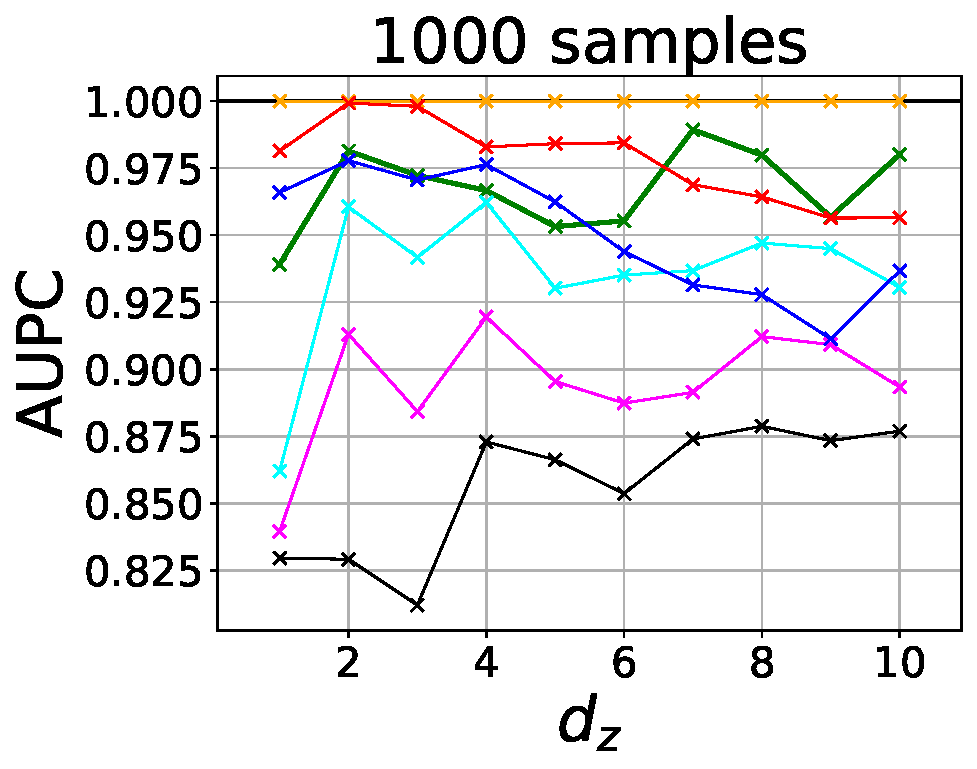
\includegraphics[height=2.2cm]{sections/appendix/independence_testing_kernel/new_figures_lap/nsamples_fixed_1000_li_dim_1_10_aupc.pdf} & 
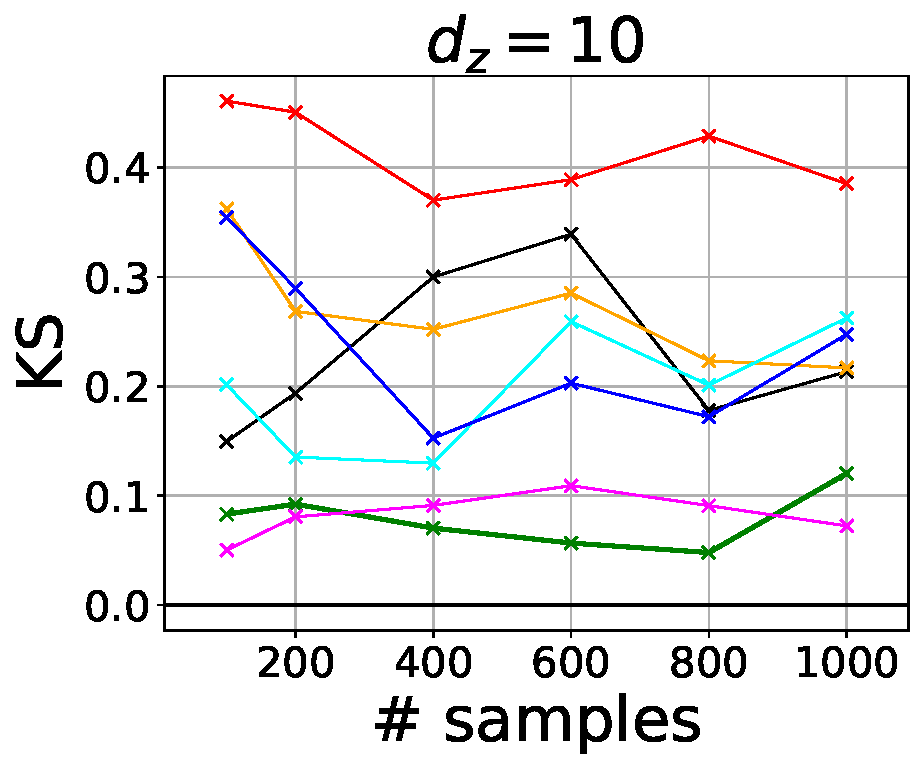
\includegraphics[height=2.2cm]{sections/appendix/independence_testing_kernel/new_figures_lap/dim_fixed_10_li_ks.pdf}& 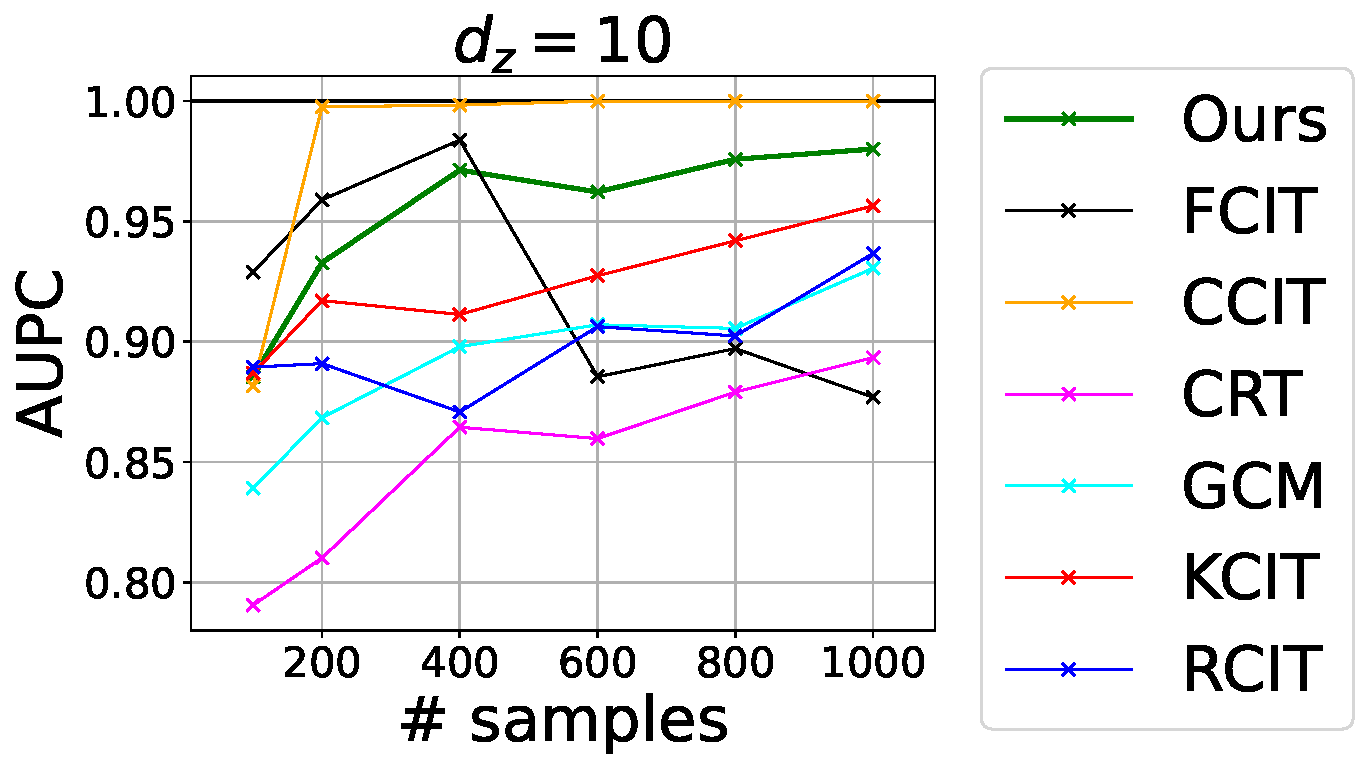
\includegraphics[height=2.2cm]{sections/appendix/independence_testing_kernel/new_figures_lap/dim_fixed_10_li_aupc.pdf} 
\end{tabular}
\caption{Comparison of the KS statistic and the AUPC of our testing procedure with other SoTA tests on the two problems presented in Eq.~\eqref{li-exp-h0} and Eq.~\eqref{li-exp-h1}  with Laplace noises. Each point in the figures is obtained by repeating the experiment for 100 independent trials. (\emph{Left, middle-left}): the KS statistic and AUPC (respectively) obtained by each test when varying the dimension $d_z$ from 1 to 10; here, the number of samples $n$ is fixed and equals to $1000$. (\emph{Middle-right, right}): the KS and AUPC (respectively), obtained by each test when varying the number of samples $n$ from 100 to 1000; the dimension $d_z$ is fixed and equals $10$.
\label{fig-exp-li-ks-laplace-supp}}
\vspace{-0.5cm}
\end{figure*}


\begin{figure*}[h]
\begin{tabular}{cccc} 
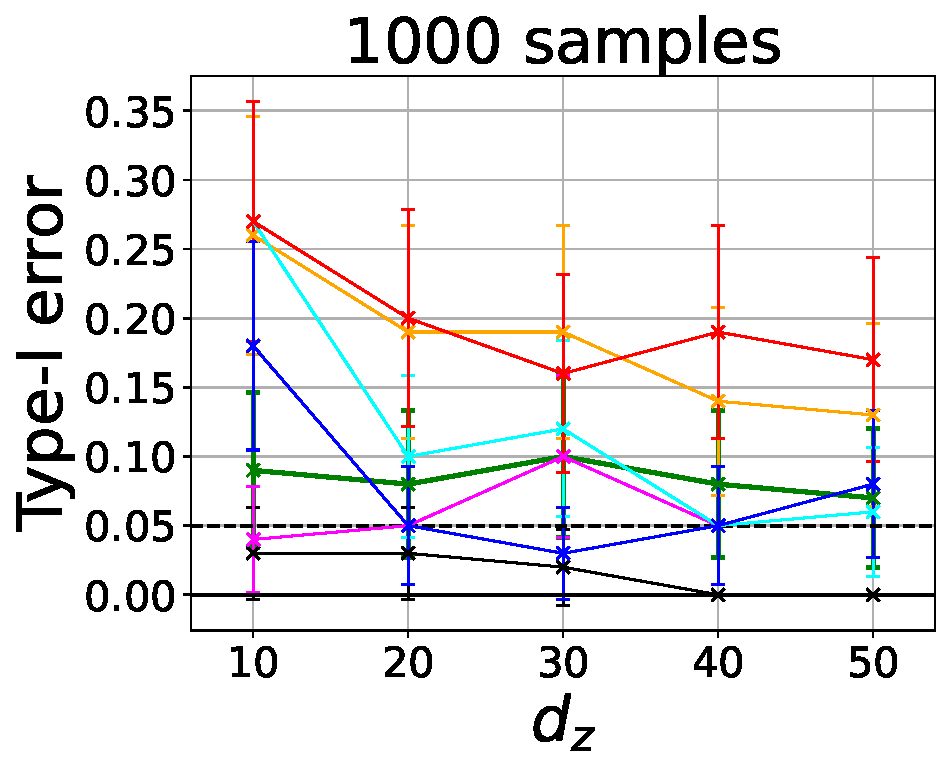
\includegraphics[height=2.2cm]{sections/appendix/independence_testing_kernel/figures_li_highdim_lap/nsamples_fixed_1000_li_dim_10_50_typeI.pdf}& 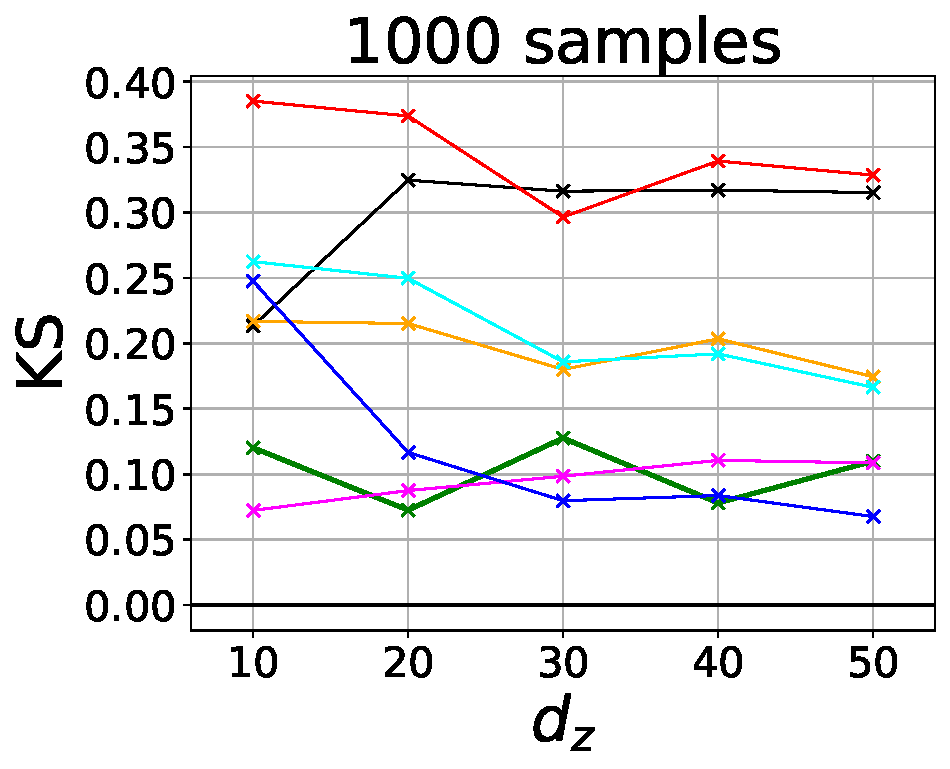
\includegraphics[height=2.2cm]{sections/appendix/independence_testing_kernel/figures_li_highdim_lap/nsamples_fixed_1000_li_dim_10_50_ks.pdf} & 
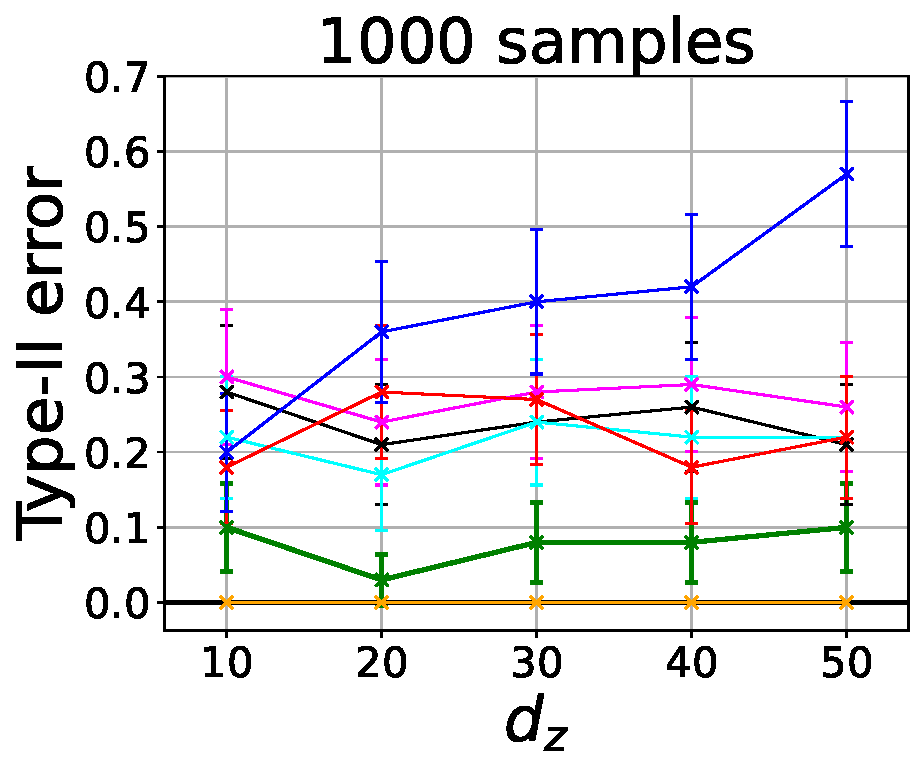
\includegraphics[height=2.2cm]{sections/appendix/independence_testing_kernel/figures_li_highdim_lap/nsamples_fixed_1000_li_dim_10_50_typeII.pdf}& \includegraphics[height=2.2cm]{sections/appendix/independence_testing_kernel/figures_li_highdim_lap/nsamples_fixed_1000_li_dim_10_50_aupc.pdf}
\end{tabular}
\caption{Comparison of the type-I error at level $\alpha=0.05$ (dashed line), type-II error (lower is better), KS statistic and the AUPC of our testing procedure with other SoTA tests on the two problems presented in Eq.~\eqref{li-exp-h0} and Eq.~\eqref{li-exp-h1} with Laplace noises. Each point in the figures is obtained by repeating the experiment for 100 independent trials. In each plot the dimension $d_z$ is varying from 10 to 50; here, the number of samples $n$ is fixed and equals to $1000$. 
\label{fig-exp-li-highdim-laplace-supp}}
\vspace{-0.8cm}
\end{figure*}










% \subsection{Additional experiments on Problems~\eqref{exp-strobl-h0} and~\eqref{exp-strobl-h1}}
% \label{sec-exp-storbl}

% \subsubsection{Gaussian Case}
% % In this section, we provide an additional comparison of the KS statistic and the AUPC obtained by the different tests when the data is generated from the models defined in Eq.~\eqref{exp-strobl-h0} and Eq.~\eqref{exp-strobl-h1}, respectively, focusing on a high dimensional setting. Figure~\ref{fig-exp-li-ks-dim} demonstrates that, in most cases, our method indeed outperforms the existing tests both in terms of the KS and AUPC performance metrics.


% \begin{figure*}[h]
% \begin{tabular}{cccc} 
% \includegraphics[height=2.2cm]{figures_strobl_gaussian/nsamples_fixed_1000_strobl_dim_1_10_typeI.pdf}& \includegraphics[height=2.2cm]{figures_strobl_gaussian/nsamples_fixed_1000_strobl_dim_1_10_typeII.pdf} & 
% \includegraphics[height=2.2cm]{figures_strobl_gaussian/dim_fixed_10_strobl_typeI.pdf}& \includegraphics[height=2.2cm]{figures_strobl_gaussian/dim_fixed_10_strobl_typeII.pdf}
% \end{tabular}
% \caption{Comparison of the type-I error at level $\alpha=0.05$ (dashed line) and the type-II error (lower is better) of our test procedure with other SoTA tests on the two problems presented in~\eqref{exp-strobl-h0} and~\eqref{exp-strobl-h1}  with Gaussian noises. Each point in the figures is obtained by repeating the experiment for 100 independent trials. (\emph{Left, middle-left}): type-I and type-II errors obtained by each test when varying the dimension $d_z$ from 1 to 10; here, the number of samples $n$ is fixed and equals to $1000$. (\emph{Middle-right, right}): type-I and type-II errors obtained by each test when varying the number of samples $n$ from 100 to 1000; here, the dimension $d_z$ is fixed and equals to $10$. 
% \label{fig-exp-strobl-type-supp}}
% \vspace{-0.5cm}
% \end{figure*}




% \begin{figure*}[ht]
% \begin{tabular}{cccc} 
% \includegraphics[height=2.2cm]{new_figures/nsamples_fixed_1000_strobl_dim_1_10_ks.pdf}& \includegraphics[height=2.2cm]{new_figures/nsamples_fixed_1000_strobl_dim_1_10_aupc.pdf} & 
% \includegraphics[height=2.2cm]{new_figures/dim_fixed_10_strobl_ks.pdf}& \includegraphics[height=2.2cm]{new_figures/dim_fixed_10_strobl_aupc.pdf} 
% \end{tabular}
% \caption{Comparison of the KS statistic (lower is better) and the AUPC (higher is better) of our testing procedure with other SoTA tests on the two problems presented in~\eqref{exp-strobl-h0} and~\eqref{exp-strobl-h1}  with Gaussian noises. Each point in the figures is obtained by repeating the experiment for 100 independent trials. (\emph{Left, middle-left}): the KS and AUPC obtained by each test when varying the dimension $d_z$ from 1 to 10, while fixing the number of samples $n$ to $1000$. (\emph{Middle-right, right}): the KS and AUPC obtained by each test when varying the number of samples $n$ from 100 to 1000, while fixing the dimension $d_z$ to $10$. These experiments show that our method outperforms other tests both in term of KS and AUPC in most of the settings.
% \label{fig-exp-strobl-supp}}
% \vspace{-0.5cm}
% \end{figure*}




% \begin{figure*}[h]
% \begin{tabular}{cccc} 
% \includegraphics[height=2.2cm]{figures_strobl_highdim_gaussian/nsamples_fixed_1000_strobl_dim_10_50_typeI.pdf}& \includegraphics[height=2.2cm]{figures_strobl_highdim_gaussian/nsamples_fixed_1000_strobl_dim_10_50_ks.pdf} & 
% \includegraphics[height=2.2cm]{figures_strobl_highdim_gaussian/nsamples_fixed_1000_strobl_dim_10_50_typeII.pdf}& \includegraphics[height=2.2cm]{figures_strobl_highdim_gaussian/nsamples_fixed_1000_strobl_dim_10_50_aupc.pdf}
% \end{tabular}
% \caption{Comparison of the type-I error at level $\alpha=0.05$ (dashed line), type-II error (lower is better), KS statistic and the AUPC of our testing procedure with other SoTA tests on the two problems presented in Eq.~\eqref{exp-strobl-h0} and Eq.~\eqref{exp-strobl-h1} with Gaussian noises. Each point in the figures is obtained by repeating the experiment for 100 independent trials. In each plot the dimension $d_z$ is varying from 10 to 50; here, the number of samples $n$ is fixed and equals to $1000$. 
% \label{fig-exp-strobl-highdim-gaussian-supp}}
% \vspace{-0.5cm}
% \end{figure*}









% \newpage


% \subsubsection{Laplace Case}







% \begin{figure*}[htb]
% \begin{tabular}{cccc} 
% \includegraphics[height=2.2cm]{new_figures_lap/nsamples_fixed_1000_strobl_dim_1_10_typeI.pdf}& \includegraphics[height=2.2cm]{new_figures_lap/nsamples_fixed_1000_strobl_dim_1_10_typeII.pdf} & 
% \includegraphics[height=2.2cm]{new_figures_lap/dim_fixed_10_strobl_typeI.pdf}& \includegraphics[height=2.2cm]{new_figures_lap/dim_fixed_10_strobl_typeII.pdf} 
% \end{tabular}
% \caption{Comparison of the type-I error at level $\alpha=0.05$ (dashed line) and the type-II error (lower is better) of our test procedure with other SoTA tests on the two problems presented in~\eqref{exp-strobl-h0} and~\eqref{exp-strobl-h1} with Laplace noises. Each point in the figures is obtained by repeating the experiment for 100 independent trials. (\emph{Left, middle-left}): type-I and type-II errors obtained by each test when varying the dimension $d_z$ from 1 to 10; here, the number of samples $n$ is fixed and equals to $1000$. (\emph{Middle-right, right}): type-I and type-II errors obtained by each test when varying the number of samples $n$ from 100 to 1000; here, the dimension $d_z$ is fixed and equals to $10$.
% \label{fig-exp-strobl-laplace-supp}}
% \vspace{-0.5cm}
% \end{figure*}




% \begin{figure*}[htb]
% \begin{tabular}{cccc} 
% \includegraphics[height=2.2cm]{new_figures_lap/nsamples_fixed_1000_strobl_dim_1_10_ks.pdf}& \includegraphics[height=2.2cm]{new_figures_lap/nsamples_fixed_1000_strobl_dim_1_10_aupc.pdf} & 
% \includegraphics[height=2.2cm]{new_figures_lap/dim_fixed_10_strobl_ks.pdf}& \includegraphics[height=2.2cm]{new_figures_lap/dim_fixed_10_strobl_aupc.pdf} 
% \end{tabular}
% \caption{Comparison of the KS statistic and the AUPC of our testing procedure with other SoTA tests on the two problems presented in Eq.~\eqref{exp-strobl-h0} and Eq.~\eqref{exp-strobl-h1}  with Laplace noises. Each point in the figures is obtained by repeating the experiment for 100 independent trials. (\emph{Left, middle-left}): the KS statistic and AUPC (respectively) obtained by each test when varying the dimension $d_z$ from 1 to 10; here, the number of samples $n$ is fixed and equals to $1000$. (\emph{Middle-right, right}): the KS and AUPC (respectively), obtained by each test when varying the number of samples $n$ from 100 to 1000; here, the dimension $d_z$ is fixed and equals to $10$.
% \label{fig-exp-strobl-ks-laplace-supp}}
% \vspace{-0.5cm}
% \end{figure*}


% \begin{figure*}[ht]
% \begin{tabular}{cccc} 
% \includegraphics[height=2.2cm]{figures_strobl_highdim_lap/nsamples_fixed_1000_strobl_dim_10_50_typeI.pdf}& \includegraphics[height=2.2cm]{figures_strobl_highdim_lap/nsamples_fixed_1000_strobl_dim_10_50_ks.pdf} & 
% \includegraphics[height=2.2cm]{figures_strobl_highdim_lap/nsamples_fixed_1000_strobl_dim_10_50_typeII.pdf}& \includegraphics[height=2.2cm]{figures_strobl_highdim_lap/nsamples_fixed_1000_strobl_dim_10_50_aupc.pdf}
% \end{tabular}
% \caption{Comparison of the type-I error at level $\alpha=0.05$ (dashed line), type-II error (lower is better), KS statistic and the AUPC of our testing procedure with other SoTA tests on the two problems presented in Eq.~\eqref{exp-strobl-h0} and Eq.~\eqref{exp-strobl-h1} with Laplace noises. Each point in the figures is obtained by repeating the experiment for 100 independent trials. In each plot the dimension $d_z$ is varying from 10 to 50; here, the number of samples $n$ is fixed and equals to $1000$.
% \label{fig-exp-strobl-highdim-laplace-supp}}
% \vspace{-0.5cm}
% \end{figure*}